\documentclass{article}
\usepackage[utf8]{inputenc}
\usepackage[a4paper, margin=2.5cm]{geometry}
\usepackage{graphicx} 
\usepackage{natbib}
\usepackage[french]{babel}

%\usepackage[default,scale=0.95]{opensans}
\usepackage[T1]{fontenc}
\usepackage{amssymb} %math
\usepackage{amsmath}
\usepackage{amsthm}
\usepackage{systeme}
\usepackage{bbm}
\usepackage{media9}
\usepackage{makecell}
\usepackage{url}
\usepackage{minted}
\usepackage{xcolor}
\usepackage{wrapfig}
\usepackage{csquotes}
\usepackage{subcaption}
\usepackage{float}
\usepackage{tikz}
\usetikzlibrary{shapes.geometric, arrows}

\tikzstyle{startstop} = [rectangle, rounded corners, 
minimum width=3cm, 
minimum height=1cm,
text centered, 
draw=black, 
fill=red!30]

\tikzstyle{io} = [trapezium, 
trapezium stretches=true, % A later addition
trapezium left angle=70, 
trapezium right angle=110, 
minimum width=3cm, 
minimum height=1cm, text centered, 
draw=black, fill=blue!30]

\tikzstyle{process} = [rectangle, 
minimum width=3cm, 
minimum height=1cm, 
text centered, 
text width=3cm, 
draw=black, 
fill=orange!30]

\tikzstyle{decision} = [diamond, 
minimum width=3cm, 
minimum height=1cm, 
text centered, 
draw=black, 
fill=green!30]
\tikzstyle{arrow} = [thick,->,>=stealth]
% \usepackage{lineno}
% \linenumbers

\usepackage{hyperref}
\hypersetup{
    % colorlinks=true,
    % linkcolor=blue,
    % filecolor=magenta,      
    % urlcolor=cyan,
    pdftitle={Projet RITAL},
    %pdfpagemode=FullScreen,
    }
\urlstyle{same} %\href{url}{Text}

\renewcommand{\baselinestretch}{1.5}


\begin{document}

\begin{titlepage}
    \begin{center}
        \vspace*{1cm}

        \Huge
        \textbf{RITAL - Projet}

        %\vspace{0.5cm}
        \LARGE
        Reconnaissance de locuteur et revues de films

        %\vspace{1.5cm}
        \Large
        Charles \textsc{Vin}, Aymeric \textsc{Delefosse}

        \vfill
        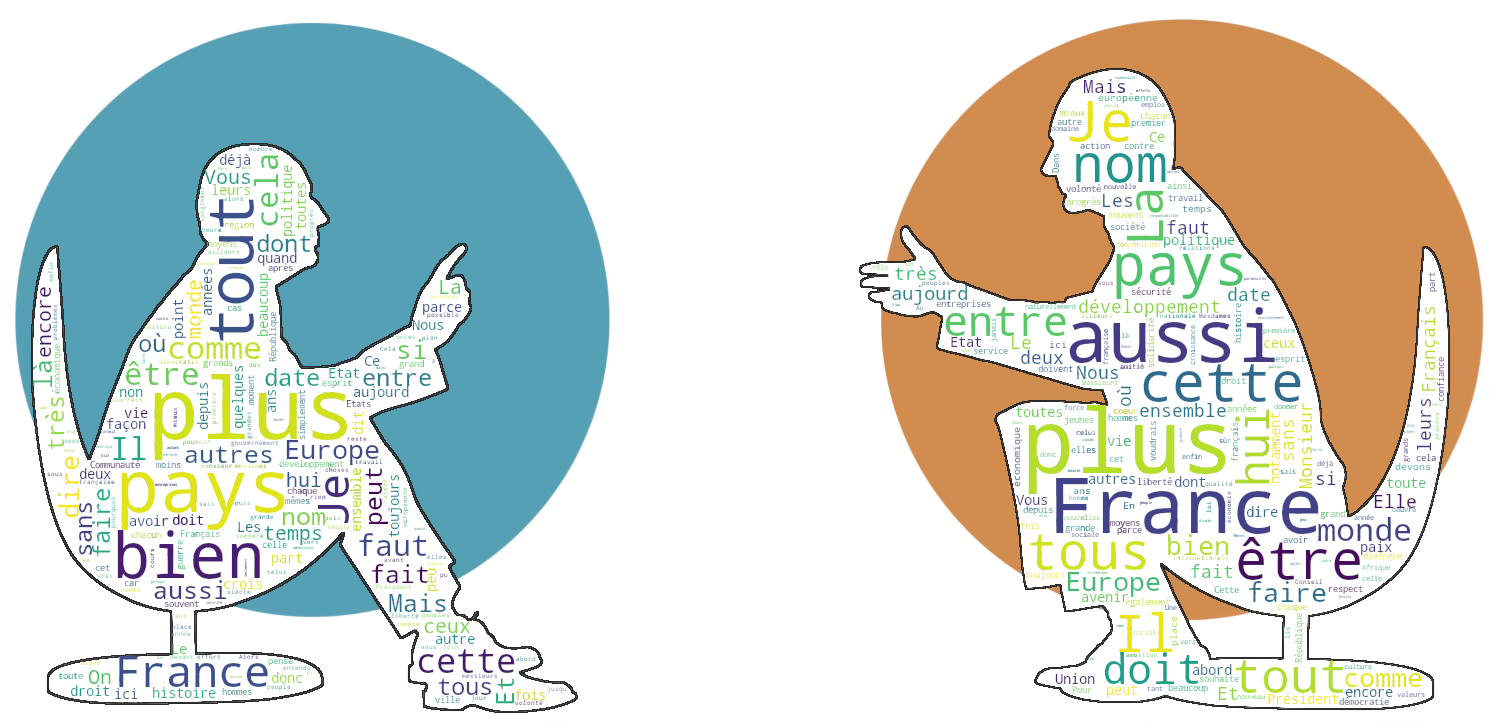
\includegraphics[width=\textwidth]{./src/locuteur/NLP.png}    
        \vfill

        \large
        DAC | 2022-2023 \hfill 
        
\includegraphics[width=0.25\textwidth]{./src/logo.png}
        \hfill
        
        
    \end{center}
\end{titlepage}

\tableofcontents
\newpage

\section{Introduction}

Le traitement du langage naturel est un domaine de recherche en informatique et en intelligence artificielle qui vise à permettre aux machines de comprendre, d'interpréter et de générer du langage ordinaire, utilisé par les êtres humains dans la communication verbale ou écrite. Dans ce contexte, notre projet consistait à réaliser du traitement du langage naturel basé sur des représentations sac de mots pour la reconnaissance de locuteur et l'analyse de sentiments. Le choix des représentations sac de mots est motivé par leur simplicité et leur efficacité pour la classification de textes.

Dans le cadre de la reconnaissance de locuteur, l'analyse s'est portée sur des phrases issues de discours prononcés par Jacques \textsc{Chirac} et François \textsc{Mitterrand}, deux anciens présidents de la République française. Ainsi, l'objectif consiste à identifier la rhétorique et de déterminer si notre approche permettait d'identifier correctement l'auteur des phrases. Pour cela, nous avons utilisé des techniques de traitement du langage naturel telles que la tokenisation et la vectorisation des textes.

L'analyse de sentiments consiste à déterminer l'orientation émotionnelle d'un texte, généralement en termes de positivité ou de négativité, ce qui est notre cas. Nous avons utilisé des critiques de films provenant de la base de données en ligne IMDb (\textit{Internet Movie Database}) pour évaluer l'efficacité de notre approche pour l'analyse de sentiments. Nous avons également utilisé des techniques de traitement du langage naturel pour prétraiter les données avant de les classifier.

Dans ce compte-rendu, nous présenterons en détail les méthodes que nous avons utilisées pour la reconnaissance de locuteur et l'analyse de sentiments, ainsi que les résultats que nous avons obtenus, dans des parties distinctes. Nous discuterons également des limites de notre approche et des perspectives d'amélioration pour de futures recherches dans ce domaine.

\section{Méthodologie}
Dans cette partie, nous allons décrire les différentes idées d'expérimentation/méthode explorées lors de ce projet. Lorsque nous discutions de ce projet, c'était très plaisant d'avoir une idée qui nous venait en tête, d'en discuter, d'anticiper les problèmes qu'elle pourrait avoir, etc. Ceci en particulier dans le cadre du problème de déséquilibre des classes dans la reconnaissance du locuteur.

\subsection{Analyses préliminaires}

Dans notre méthodologie, une étape importante est l'exploration préliminaire des jeux de données pour comprendre la nature de notre vocabulaire.

La première question que nous abordons est la taille d'origine du vocabulaire. Nous examinons le nombre total de mots uniques dans nos jeux de données pour avoir une idée de la complexité de la tâche de traitement du langage naturel. Cette information peut également être utile pour l'optimisation du modèle en réduisant la taille du vocabulaire, par exemple. Nous poursuivons ensuite notre exploration préliminaire en nous demandant quels sont les 100 mots les plus fréquents, que nous visualiserons à l'aide de nuages de mots. Ensuite, nous examinons la distribution d'apparition des mots en utilisant la loi de Zipf. Cette loi montre que quelques mots sont très fréquents, tandis que la majorité des mots sont rares. En comprenant cette distribution, nous pouvons identifier les mots clés qui peuvent être les plus importants dans notre modèle. Enfin, nous examinons les bigrammes et les trigrammes les plus fréquents, ce qui peut nous donner une idée des relations entre les mots dans nos jeux de données. Cela peut nous aider à mieux comprendre la structure des phrases dans nos jeux de données et nous aider à concevoir un modèle plus précis. 

En effet, les $n$-grammes sont une technique d'analyse de texte qui consiste à diviser le texte en séquences de $n$ mots consécutifs. Les $n$-grammes peuvent être utilisés pour capturer des informations sur la structure linguistique d'un texte, comme les relations entre les mots ou les phrases. Les $n$-grammes les plus couramment utilisés sont les unigrammes ($n = 1$), les bigrammes ($n = 2$) et les trigrammes ($n = 3$). L'utilisation de $n$-grammes dans l'analyse de texte permet d'obtenir des modèles plus précis, car ils prennent en compte l'ordre des mots et des phrases, contrairement aux approches de représentation de texte basées sur des sacs de mots. Cependant, l'utilisation d'un nombre de $n$-grammes plus élevé peut entraîner une augmentation de la complexité computationnelle et peut nécessiter un ensemble de données plus important pour obtenir des résultats significatifs.

En résumé, l'exploration préliminaire de nos jeux de données est une étape essentielle dans l'extraction du vocabulaire pour le traitement du langage naturel. En examinant la taille d'origine du vocabulaire, les mots les plus courants, la distribution des mots et les bigrammes/trigrammes les plus fréquents, nous pouvons mieux comprendre la complexité de notre tâche et optimiser notre modèle pour de meilleurs résultats.

\subsection{Cadre de travail}
Il existait de nombreuses possibilités et tâches à réaliser. La première idée qui nous est venue consistait à créer un ensemble de fonctions d'utilité pour entraîner, évaluer et comparer différents modèles avec des paramètres différents, tout en enregistrant les résultats dans un fichier CSV pour une visualisation ultérieure. Cette partie a été conçue dans l'optique de comparer les performances des nombreux pré-traitements possibles.
Dans ce but, nous avons créé des fonctions pour charger les données, charger une configuration de pré-traitements et créer une fonction d'analyse pour celle-ci, adapter et évaluer plusieurs modèles sur cette configuration, puis sauvegarder les résultats dans un CSV.

Cependant, l'utilité de tout cela s'est avérée limitée, car les pipelines de Scikit-learn peuvent généralement réaliser les mêmes tâches de manière équivalente. Les pipelines sont des outils qui permettent de chaîner des étapes de traitement de données, ce qui automatise le flux de travail, simplifie le code et facilite la répétabilité de l'analyse. Par exemple, la pipeline suivante transforme les données en entrées en une représentation sac de mots, puis les pondère sous une représentation TF-IDF, avant de fit le tout sur un modèle de régression logistique. Il est par ailleurs possible de désactiver la pondération TF-IDF en changeant les paramètres de cet objet.

\begin{center}
\begin{tikzpicture}[node distance=2cm]

\node (pro1) [process] {CountVectorizer};
\node (pro2) [process, below of=pro1] {TfidfTransformer};
\node (pro3) [process, below of=pro2] {LogisticRegression};

\draw [arrow] (pro1) -- (pro2);
\draw [arrow] (pro2) -- (pro3);

\end{tikzpicture}
\end{center}

Malgré cela, deux cas d'utilisation de ces différents codes sont restés pertinents : la fonction \\ \color{blue} \texttt{print\_score(y\_true, y\_hat)}\color{black}, qui affiche toutes les mesures de performance possibles, est restée utile tout au long du projet. L'autre cas d'utilisation, malheureusement non testé, était l'emploi du framework pour l'évaluation des pré-traitements dans une recherche de grille (GridSearch). Cette méthode aurait permis d'évaluer l'impact du stemming ou de la lemmatisation, qui n'est pas implémenté dans les \color{blue} Vectorizers \color{black} de Scikit Learn.

\subsection{Estimations des performances}

Les classifieurs choisis pour réaliser notre modèle sont : la classification naïve bayésienne, la régression logistique et le SVM linéaire. Pour évaluer nos modèles, nous aurons besoin de choisir des fonctions de scoring pertinentes, mais lesquelles choisir ? Accuracy, précision, rappel... ? Notre choix s'est arrêté sur le F1-Score et le ROC-AUC. Le F1-Score, qui est la moyenne harmonique de la précision et du rappel (recall), est une mesure qui prend en compte les deux aspects de la performance : la capacité à identifier correctement les vrais positifs et à minimiser les faux positifs. De même, le ROC-AUC (Area Under the Receiver Operating Characteristic Curve) est une mesure de performance qui prend en compte le taux de vrais positifs (TPR) et le taux de faux positifs (FPR). Elle permet d'évaluer la performance du modèle sur l'ensemble de la courbe ROC, plutôt que sur un seul point de seuil de classification. En somme, le F1-Score et le ROC-AUC sont des métriques de performance fiables pour évaluer la qualité des modèles de classification sur des données déséquilibrées (ou non). 

Ainsi, avant de nous lancer dans des grandes recherches, nous avons effectués des estimations supplémentaires à l'aide de modèles non paramétrés, comme par exemple les performances, le temps d'apprentissage et le score obtenu en fonction de la taille des données d'entraînement, à quelles performances s'attendre en fonction de la taille des données d'entraînement, combien de folds choisir pour la cross-validation, etc.

\subsection{Entraînement des modèles}

De plus, pour les deux tâches, les données à notre disposition représentent notre seule source d'entrée pour entraîner nos données : nous n'avons pas de données de validation. Les données de validation étant un ensemble de données distinct de l'ensemble d'entraînement utilisé pour former le modèle, il est utilisé pour évaluer les performances du modèle sur des données qu'il n'a jamais vues auparavant. Ainsi, son absence peut rendre difficile l'estimation des performances du modèle sur de nouvelles données, entraînant une sélection de modèle inadéquate ou une optimisation de paramètres biaisée. Cependant, cette caractéristique représente l'enjeu principal du projet et de la construction de notre \textit{baseline} : il faut être capable d'estimer les performances de généralisation du modèle à partir des données d'entraînement.

Si nous n'avons pas de données de validation, nous pouvons envisager d'utiliser des techniques telles que la validation croisée pour estimer les performances de notre modèle. La validation croisée consiste à diviser les données en plusieurs ensembles d'entraînement et de validation, puis à entraîner et évaluer le modèle plusieurs fois sur différentes combinaisons d'ensembles. Cela permet d'obtenir une estimation plus fiable des performances du modèle en utilisant toutes les données disponibles.

Cependant, il est important de noter que la validation croisée est plus coûteuse en termes de temps de calcul, car elle nécessite plusieurs entraînements et évaluations du modèle, et peut également réduire le nombre de données disponibles pour l'entraînement, ce qui peut affecter les performances du modèle. De plus, plusieurs questions se posent : la validation croisée est-elle nécessaire ? Un simple \textit{split} sur les données d'entraînement est-il suffisant ? Combien de blocs choisir pour avoir une validation croisée stable ? 

Mais, nous pouvons dores et déjà commencer à y répondre :  la validation croisée est essentielle pour garantir que le modèle est performant et généralise bien sur des données inconnues. Sans, impossible de s'assurer que le modèle généralise bien sur des données inconnues. Elle permet également de réduire le risque de sur-apprentissage et de sélectionner les paramètres du modèle de manière plus fiable en utilisant une approche plus rigoureuse.

\subsection{Comparaison et sélection des modèles}

Après avoir effectué ses estimations, nous nous sommes attelés à la recherche du meilleur modèle et de la meilleure représentation sac de mots. Il est courant de procéder par une recherche d'hyperparamètres et une validation croisée. Tout d'abord, il est important de choisir un ensemble de modèles potentiels à tester. Ensuite, on peut fixer un certain nombre d'hyperparamètres pour chaque modèle et les ajuster en utilisant une méthode de recherche d'hyperparamètres telle que la recherche aléatoire ou la recherche en grille (\textit{gridsearch}). 

Ensuite, on peut comparer les performances de chaque modèle et de chaque représentation Bag of Words (par exemple, unigrammes, bigrammes, etc.) et choisir celui qui a le meilleur score de validation croisée. Il est important de garder à l'esprit que le meilleur modèle et la meilleure représentation Bag of Words peuvent varier en fonction du jeu de données et des objectifs spécifiques du projet. Une autre méthode est la recherche aléatoire, où les valeurs des hyperparamètres sont choisies de manière aléatoire dans un intervalle prédéfini. Cette méthode est moins coûteuse que la recherche par grille, mais peut ne pas couvrir tout l'espace de recherche. Enfin, il existe des méthodes plus avancées telles que l'optimisation bayésienne ou la recherche par sur-échantillonnage (hyperband), qui permettent de trouver rapidement les hyperparamètres optimaux en utilisant des modèles probabilistes.

A l'origine, nous avions décidé d'effectuer une gridsearch pure, mais c'est un processus très coûteux qui peut mettre des dizaines d'heures. C'est pourquoi nous avons décidé pour une recherche aléatoire par échantillonnage. Cela consiste en une sélection aléatoire d'hyperparamètres, suivie d'une sélection itérative des meilleurs hyperparamètres et de l'élimination des moins performants. L'algorithme commence par sélectionner un grand nombre de combinaisons aléatoires d'hyperparamètres, puis il les évalue sur une petite fraction de l'ensemble des données. Les meilleures configurations sont sélectionnées pour la prochaine ronde d'évaluation, tandis que les moins performantes sont éliminées. Ce processus se répète jusqu'à ce qu'il ne reste plus qu'un petit nombre de configurations, qui sont ensuite évaluées sur l'ensemble complet des données. Cela permet d'éviter de gaspiller des ressources sur des combinaisons moins performantes et d'accélérer considérablement la recherche. Ainsi, nous avons lancé des expériences sur nos propres machines mais également sur les machines de l'université, en SSH, sous \texttt{screen} pour pouvoir se déconnecter de la session SSH en s'assurant que notre recherche continue de tourner (sauf s'il y a une coupure d'électricité, ou un crash de l'ordinateur, ce qui est arrivé).

\section{Reconnaissance de locuteur}

Nous avons affaire à diverses allocutions prononcées lors de différentes prises de parole publiques par Jacques \textsc{Chirac} et François \textsc{Mitterrand}. Un exemple de phrases que l'on peut lire dans nos données :

\begin{displayquote}
\og Une autre urgence est celle qui découle des nouvelles technologies, de la rencontre entre la linguistique et l'informatique, du dialogue entre la voie humaine et la machine. Le traitement informatique des langues progresse à vive allure. [...] La rencontre des nouvelles techniques de l'informatique et de la linguistique transforme une discipline jusque là seulement "littéraire" [...] en une science appliquée, la linguistique automatique. \fg  
\end{displayquote}
--- Allocution de M. François Mitterrand, Président de la République, sur le rôle de l'Académie française en matière de création et de terminologie linguistique et le traitement informatique des langues, Paris, le 12 décembre 1985.


\subsection{Données}

Le jeu de données est constitué de 57~413 lignes (une ligne étant une phrase). Les phrases ont été préalablement étiquetées avec le nom du locuteur ("M" pour Mitterrand (encodée à -1), "C" pour Chirac (encodée à 1)). 49~890 (89.87 \%) phrases sont étiquetées "C"  et 7~523 (13.10 \%) "M". Ainsi, un premier constat majeur est que les données présentent un déséquilibre très important : presque 9 phrases sur 10 sont prononcées par Jacques \textsc{Chirac} et représente une discussion majeure de cette partie. En effet, le déséquilibre des données est un problème courant en \textit{machine learning} et est un problème reconnu comme dur dans la communauté. 

Dans notre contexte, à savoir un problème de classification binaire, si une classe est beaucoup plus représentée que l'autre (ici "C"), cela peut conduire à une forte inclinaison du modèle vers la classe majoritaire, ce qui peut compromettre les performances du modèle sur la classe minoritaire.

Il est donc important de prendre en compte ce déséquilibre lors de la préparation des données et de la sélection des algorithmes d'apprentissage automatique pour obtenir des résultats précis et fiables. Des techniques telles que le sur-échantillonnage de la classe minoritaire, le sous-échantillonnage de la classe majoritaire, la génération de données synthétiques ou encore l'utilisation d'algorithmes d'apprentissage automatique adaptés peuvent être utilisées pour résoudre ce problème, ce que nous avons étudié. Le déséquilibre des données peut également être évalué à l'aide de mesures telles que la précision, le rappel, le score F1 et l'AUC (aire sous la courbe), qui permettent d'évaluer la capacité du modèle à prédire avec précision les classes minoritaires.

% ptit graphique


\subsection{Analyses}

Dans un premier temps, et comme expliqué en méthodologie, nous effectuons des analyses préliminaires sur notre jeu de données, pour mieux le comprendre. Nous afficherons plusieurs scénarios : les 1000 mots les plus fréquents et leur loi de Zipf associée (figures \ref{zipfs_nostopwords_pres} et \ref{wordcloud_nostopwords_pres}), les 1000 mots les plus fréquents après avoir supprimé les stopwords (figures \ref{zipfs_stopwords_pres} et \ref{wordcloud_stopwords_pres}), les mots les plus fréquents par classe (figure \ref{president_dataviz}) ou encore un tableau récapitulatif des 20 mots les plus fréquents (table \ref{tab_pres}).

\paragraph{Stopwords}
Les mots vides (stopwords) sont des mots courants et généralement peu significatifs pour la tâche de traitement du langage naturel, tels que "le", "la", "et", "de", etc. Leur présence dans le corpus de texte peut avoir un impact négatif sur la qualité du modèle en introduisant du bruit et en réduisant la précision de l'analyse. Avec ces mots, nous avons un vocabulaire composé de 28~524 mots pour un total de 1~205~104 mots.

\begin{figure}[H]
    \centering
    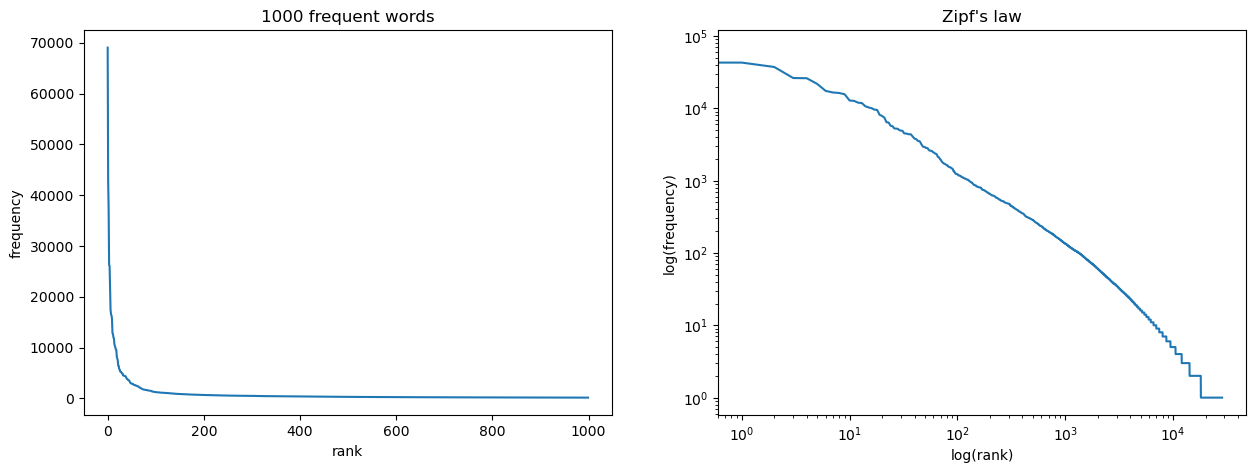
\includegraphics[width=\textwidth]{./src/locuteur/zipfs_nostopwords.png}
    \caption{Vocabulaire, avec stopwords}
    \label{zipfs_nostopwords_pres}
\end{figure}

\begin{figure}[H]
    \centering
    \begin{minipage}[b]{0.45\textwidth}
        \centering
        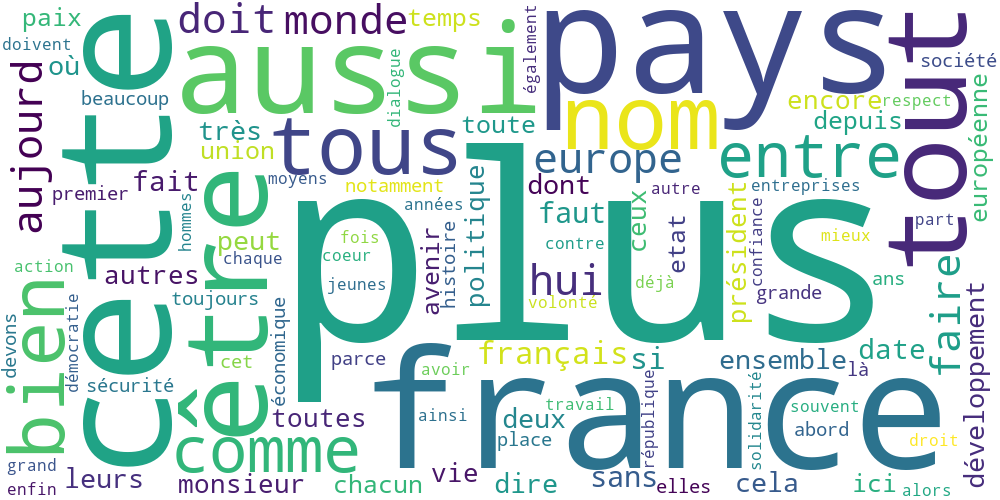
\includegraphics[width=\textwidth]{./src/locuteur/wordcloud_stopwords.png}
        \caption{Nuage de mots (top 100), sans stopwords}
        \label{wordcloud_stopwords_pres}
    \end{minipage}
    \hfill
    \begin{minipage}[b]{0.45\textwidth}
        \centering
        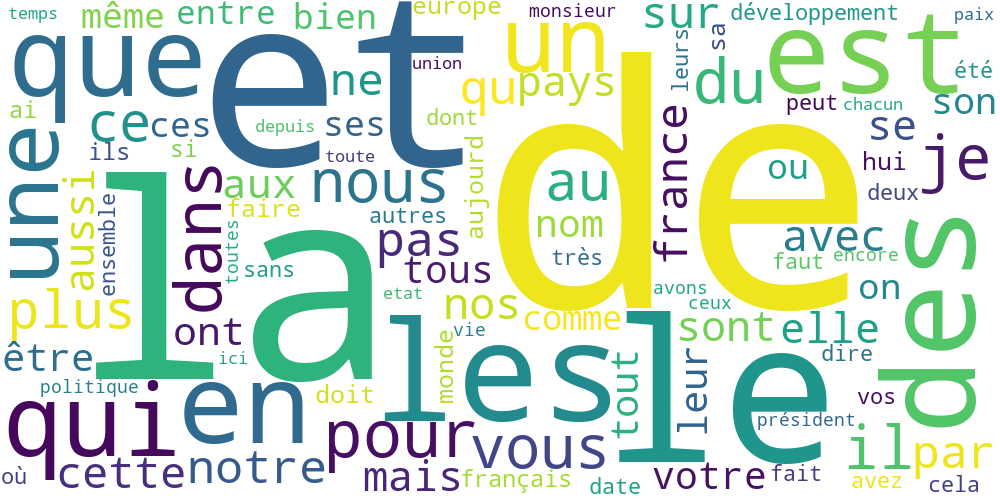
\includegraphics[width=\textwidth]{./src/locuteur/wordcloud_nostopwords.png}
        \caption{Nuage de mots (top 100), avec stopwords}
        \label{wordcloud_nostopwords_pres}
    \end{minipage}
\end{figure}

Cependant, leur suppression peut également avoir des conséquences. En effet, certains stopwords peuvent avoir une signification particulière dans certaines tâches de traitement du langage naturel, comme la reconnaissance d'entités nommées ou la détection de polarité dans les sentiments. Par conséquent, il est important de bien comprendre la tâche en question avant de décider de supprimer ou non les stopwords. Sans les stopwords, nous avons un vocabulaire qui passe à 28 400 mots pour 673 679 au total (soit une réduction par 2 du nombre total de mots).

\begin{figure}[H]
    \centering
    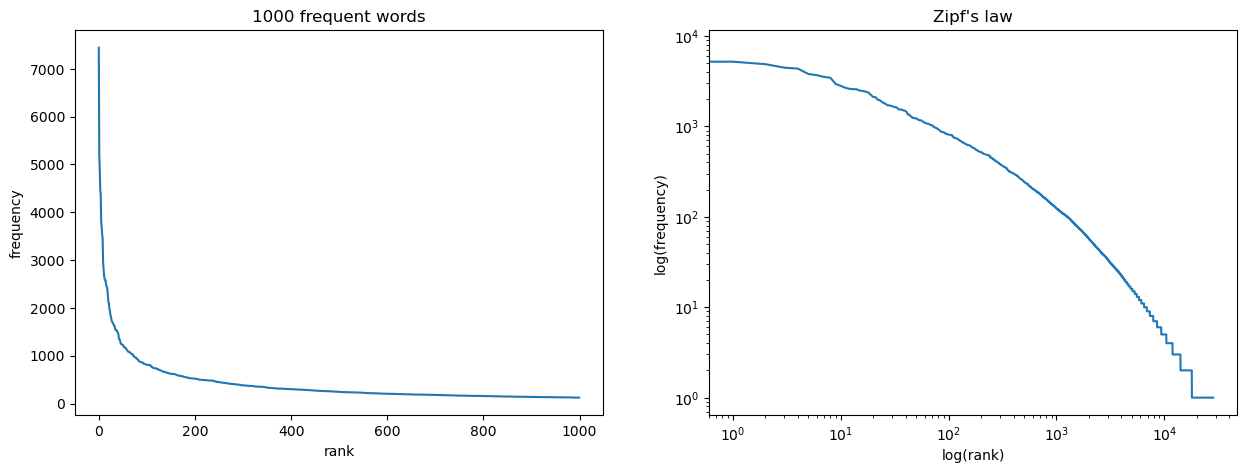
\includegraphics[width=\textwidth]{./src/locuteur/zipfs_stopwords.png} 
    \caption{Vocabulaire, sans stopwords}
    \label{zipfs_stopwords_pres}
\end{figure}


Il est également important de regarder le vocabulaire utilisé pour chacune de nos classes (figure \ref{president_dataviz}), qui nous permettrait d'identifier potentiellement des mots significatifs pour la construction des poids du modèle (sous la forme d'une jolie data visualisation réalisée grâce au package \texttt{wordcloud}). 

\begin{figure}[!htpb]
    \centering
    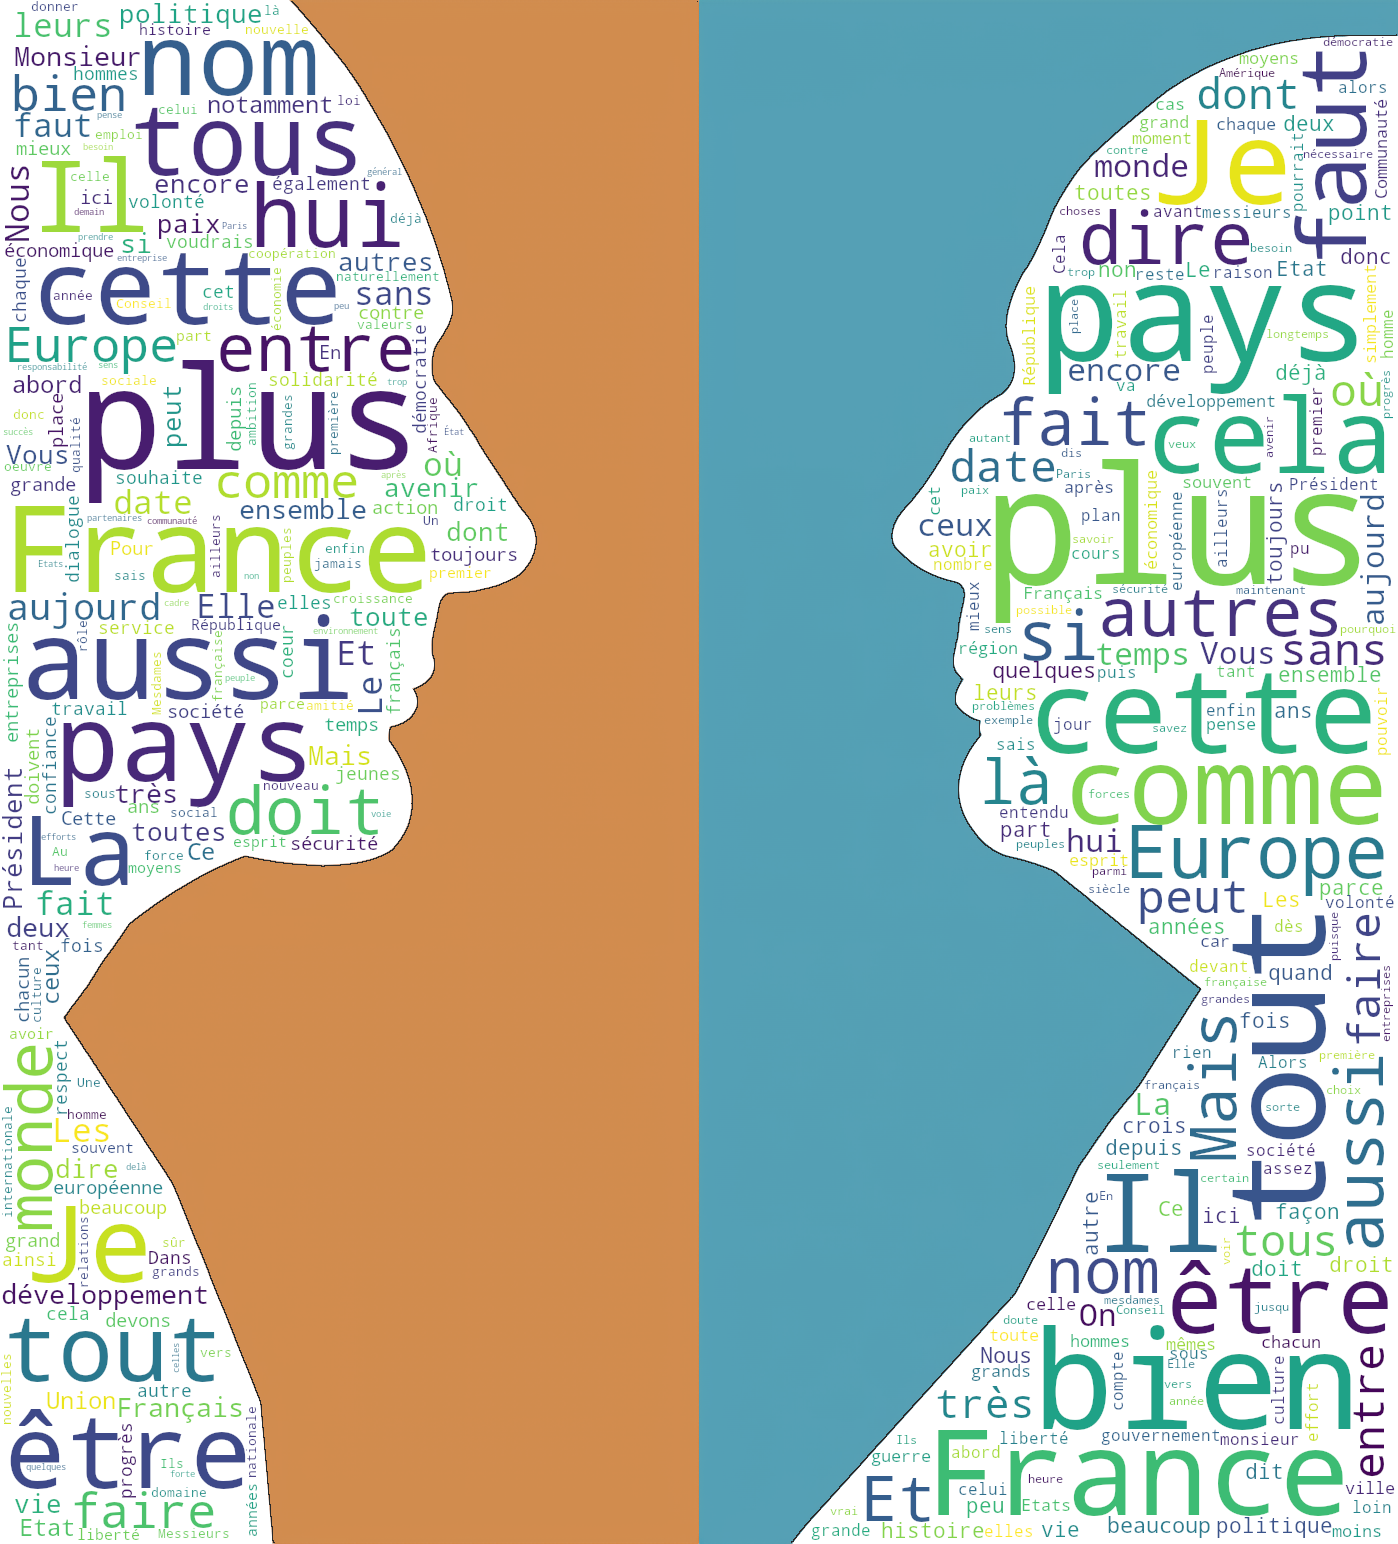
\includegraphics[width=\textwidth]{./src/locuteur/president_dataviz.png} 
    \caption{Les 200 mots les plus prononcés par Chirac et Mitterrand, sans stopwords}
    \label{president_dataviz}
\end{figure}

Dans l'ensemble, l'impact des stopwords sur le traitement du langage naturel dépend de la tâche en question et il est important de bien comprendre les implications de leur suppression avant de prendre une décision. Un récapitulatif des 20 mots les plus fréquents, avec ou sans stopwords, et leur fréquence associée.

\begin{table}[H]
\centering
\begin{subtable}{0.45\linewidth}
\centering
\begin{tabular}{|c|c|}
\hline
\textbf{Mot} & \textbf{Fréquence} \\
\hline
de & 69031 \\
la & 42863 \\
et & 37281 \\
le & 26219 \\
les & 26067 \\
des & 21768 \\
est & 17401 \\
en & 16553 \\
que & 16292 \\
qui & 15635 \\
un & 12815 \\
une & 12669 \\
pour & 11964 \\
dans & 11820 \\
du & 10659 \\
je & 10286 \\
il & 10037 \\
nous & 9590 \\
vous & 9499 \\
au & 8122 \\
\hline
\end{tabular}
\caption{20 mots les plus fréquents (avec stopwords)}
\end{subtable}
\hfill
\begin{subtable}{0.45\linewidth}
\centering
\begin{tabular}{|c|c|}
\hline
\textbf{Mot} & \textbf{Fréquence} \\
\hline
plus & 7443 \\
france & 5201 \\
cette & 4883 \\
pays & 4464 \\
aussi & 4366 \\
être & 3808 \\
tout & 3688 \\
nom & 3530 \\
tous & 3457 \\
bien & 2945 \\
comme & 2811 \\
entre & 2678 \\
europe & 2609 \\
hui & 2582 \\
aujourd'hui & 2581 \\
monde & 2492 \\
doit & 2463 \\
faire & 2426 \\
français & 2371 \\
si & 2231 \\
\hline
\end{tabular}
\caption{20 mots les plus fréquents (sans stopwords)}
\end{subtable}
\caption{Comparaison des 20 mots les plus fréquents avant et après suppression des stopwords}
\label{tab_pres}
\end{table}

\begin{figure}[H]
    \centering
    \begin{minipage}[b]{0.45\textwidth}
        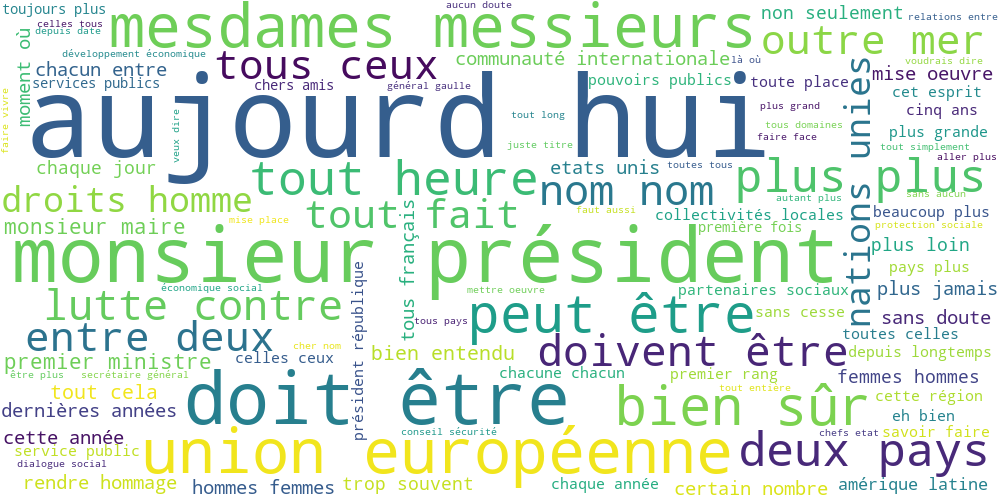
\includegraphics[width=\textwidth]{./src/locuteur/wordcloud_stopwords_2grams.png} 
        \caption{Nuage de mots (top 100), bi-grammes, sans stopwords}
        \label{wordcloud_stopwords_2grams}
    \end{minipage}
    \hfill
    \begin{minipage}[b]{0.45\textwidth}
        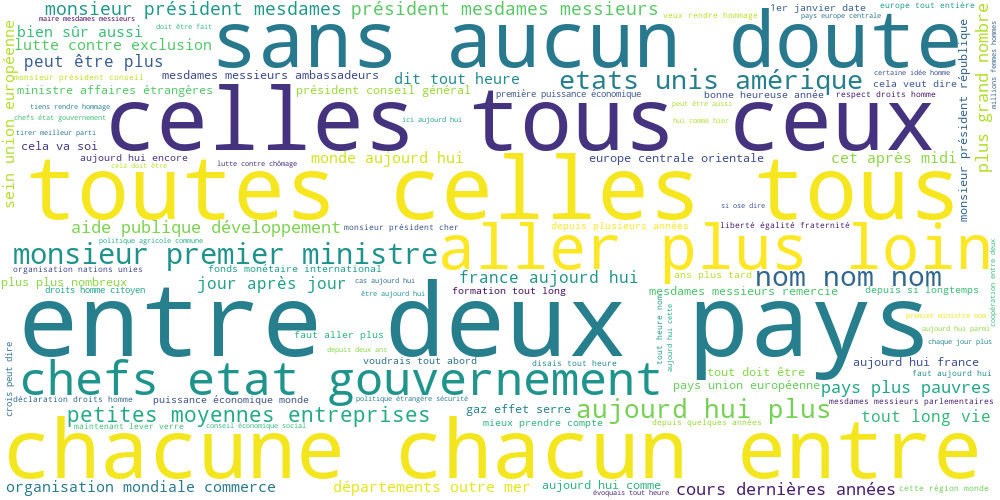
\includegraphics[width=\textwidth]{./src/locuteur/wordcloud_stopwords_3grams.png} 
        \caption{Nuage de mots (top 100), tri-grammes, sans stopwords}
        \label{wordcloud_stopwords_3grams}
    \end{minipage}
\end{figure}

\paragraph{Et les $n$-grammes ?}

On voit bien que les $n$-grammes apportent un tout nouveau regard sur les données, et nous incorporerons donc les $n$-grammes dans notre recherche de meilleur modèle.

\subsection{Estimations}

\subsubsection{Temps d'apprentissage}
Avec ces informations à l'esprit, nous avons effectué des estimations supplémentaires à l'aide de modèles non paramétrés avant de nous lancer dans des enquêtes à grande échelle. En premier, nous nous sommes demandés : à quelles performances s'attendre en fonction de la taille des données d'entraînement (figure \ref{learningcurve_pres}) ? Comment évoluent les temps d'apprentissage et de notation (figure \ref{complexity_analysis_nsamples_pres}) ? Y'a-t-il un compromis entre l'augmentation du temps d'apprentissage et le score obtenu par validation croisée (figure \ref{complexity_analysis_accuracy_pres}) ?

\begin{figure}[H]
    \centering
    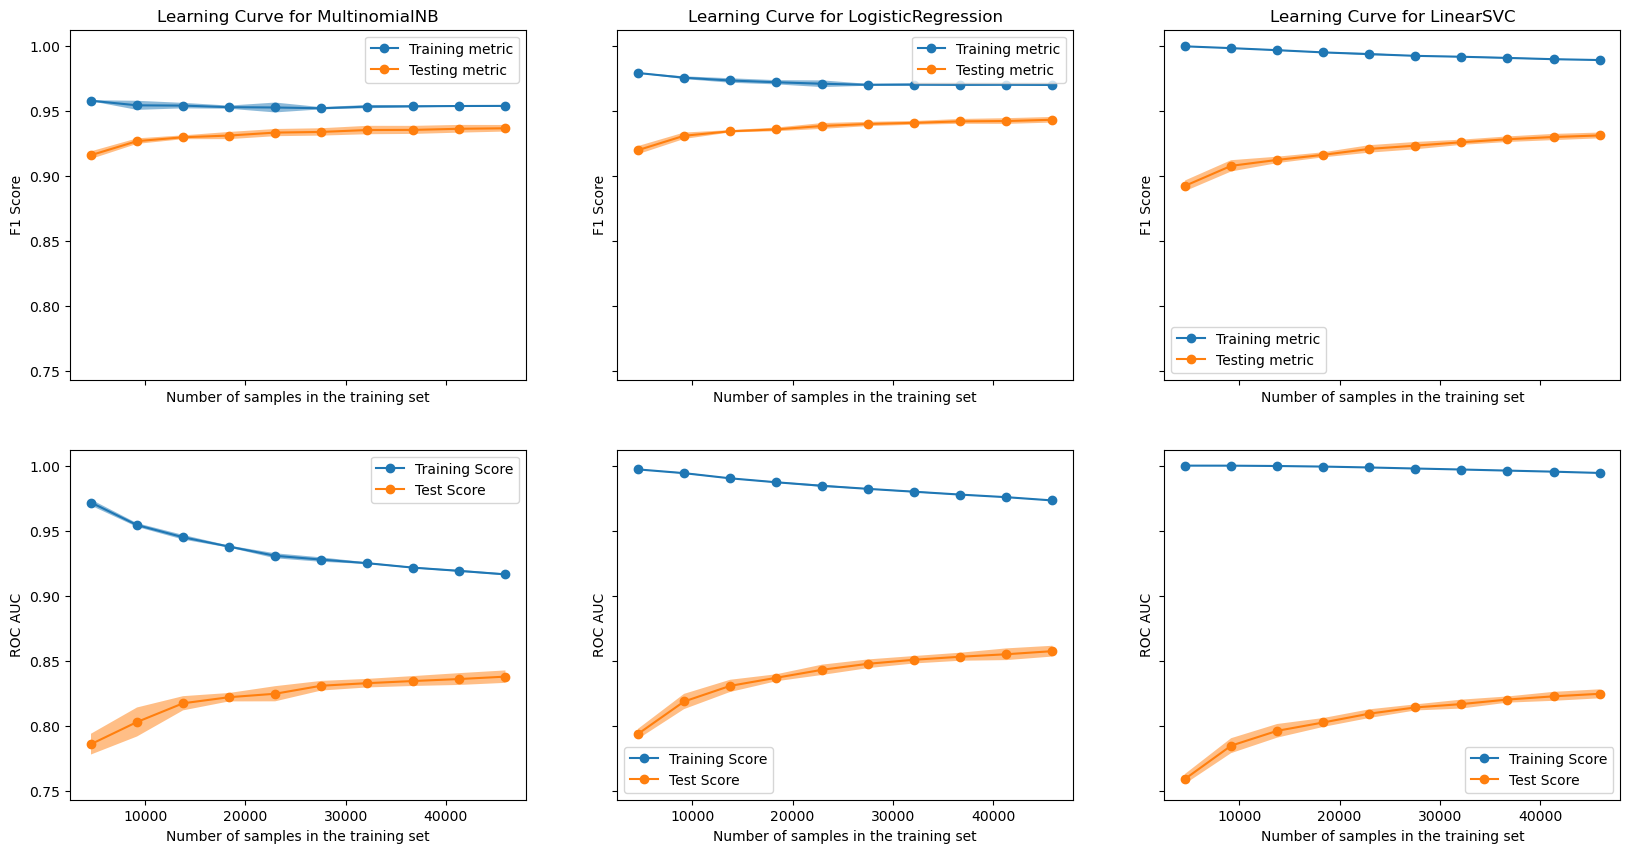
\includegraphics[width=\textwidth]{./src/locuteur/learningcurve.png} 
    \caption{Courbes d'apprentissage}
    \label{learningcurve_pres}
\end{figure}

Nous commençons par analyser la courbe d'apprentissage du classificateur Bayésien naïf. Sa forme est souvent observée dans des jeux de données plus complexes : le score d'entraînement est élevé lorsqu'on utilise peu d'échantillons pour l'entraînement, puis diminue lorsqu'on augmente le nombre d'échantillons, tandis que le score de test est très faible au début puis augmente lorsqu'on ajoute des échantillons. Les scores d'entraînement et de test deviennent plus réalistes lorsque tous les échantillons sont utilisés pour l'entraînement.

Nous observons une autre courbe d'apprentissage typique pour la régression logistique et un SVM avec un noyau linéaire. Le score d'entraînement reste élevé quelle que soit la taille de l'ensemble d'entraînement. En revanche, le score de test augmente avec la taille de l'ensemble d'entraînement. En effet, il augmente jusqu'à un certain point où il atteint un plateau. Observer un tel plateau est une indication qu'il pourrait ne pas être utile d'acquérir de nouvelles données pour entraîner le modèle car les performances de généralisation du modèle ne s'amélioreront plus.

\begin{figure}[H]
    \centering
    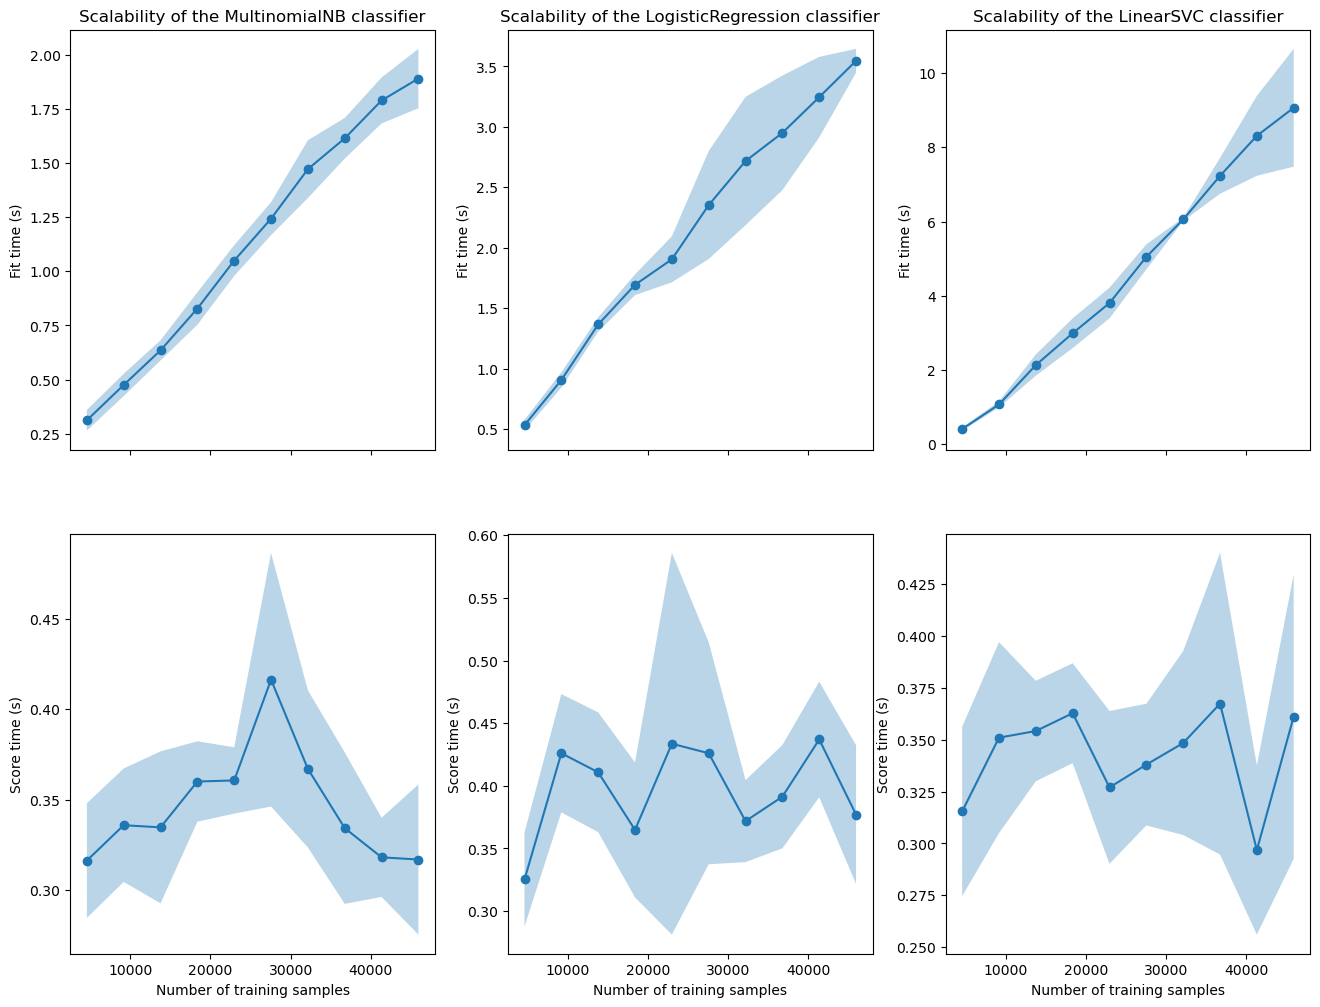
\includegraphics[width=\textwidth]{./src/locuteur/complexity_analysis_nsamples.png} 
    \caption{Evolutivité des classifieurs en fonction de la taille des données d'entraînement}
    \label{complexity_analysis_nsamples_pres}
\end{figure}

Nous constatons que l'évolutivité de nos 3 classificateurs est très similaire. La complexité au moment de l'ajustement et du score augmente rapidement avec le nombre d'échantillons. Cela n'est pas étonnant pour la régression logistique et le SVM, car la complexité du temps d'ajustement de ce classificateur est de l'ordre quadratique avec le nombre d'échantillons, ce qui rend difficile l'évolutivité vers des ensembles de données de plus de quelques dizaines de milliers d'échantillons. Cependant, les résultats obtenus pour le classificateur Bayésien naïf étonnent, car c'est un classificateur qui est connu pour s'échelonner beaucoup mieux avec une complexité plus faible au moment de l'ajustement et du score. 

\begin{figure}[H]
    \centering
    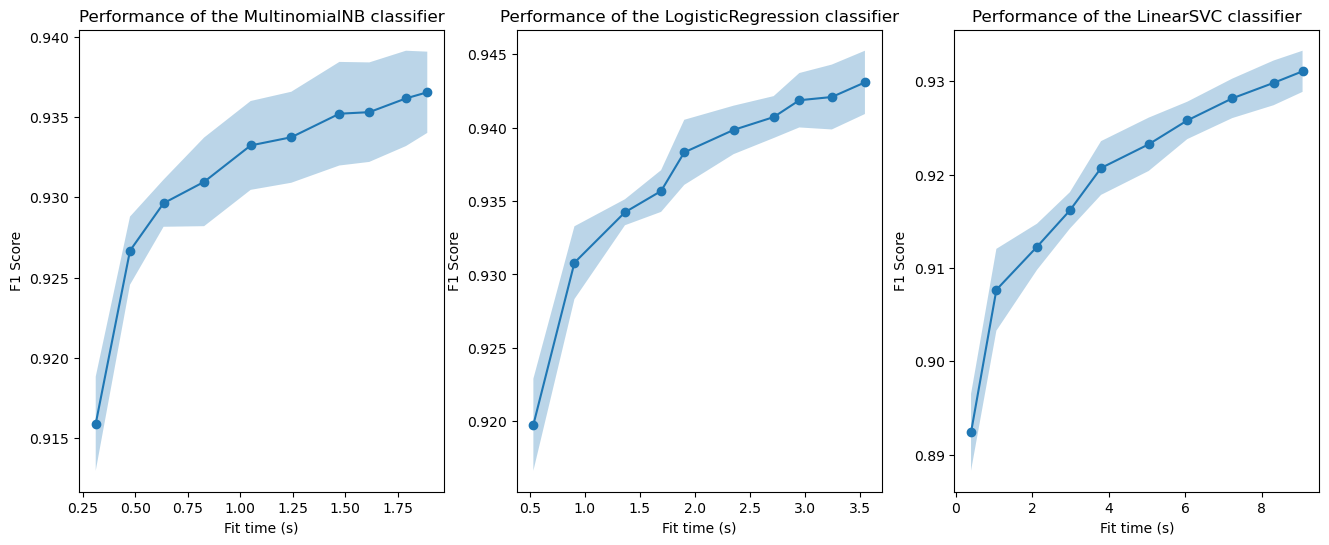
\includegraphics[width=\textwidth]{./src/locuteur/complexity_analysis_accuracy.png} 
    \caption{Performance des classifieurs}
    \label{complexity_analysis_accuracy_pres}
\end{figure}

Et enfin, on compare le temps d'apprentissage par rapport à la taille du vocabulaire utilisé (figure \ref{complexity_analysis_vocabulary}) : ici, les résultats ne sont pas étonnants et on voit bien que la taille du vocabulaire n'a aucune influence sur la complexité du classifieur Bayésien naïf. Cependant, contrairement à précédemment, la complexité de la régression logistique est beaucoup plus grande que le SVM, alors que précédemment c'était l'inverse.

\begin{figure}[H]
    \centering
    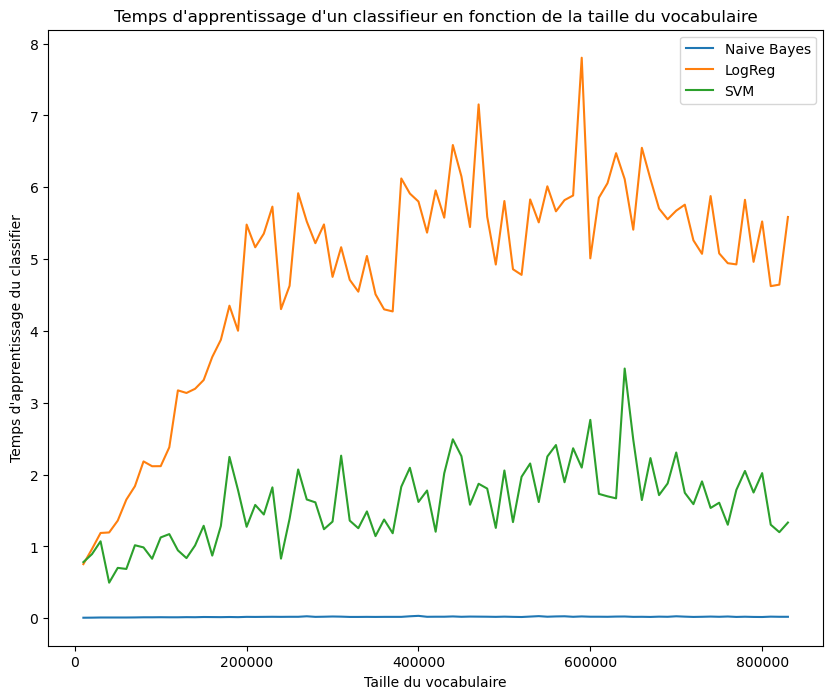
\includegraphics[width=0.6\textwidth]{./src/locuteur/complexity_analysis_vocabulary.png} 
    \caption{Evolutivité des classifieurs en fonction de la taille du vocabulaire}
    \label{complexity_analysis_vocabulary}
\end{figure}

Les $n$-grammes auront donc un impact important sur nos temps d'apprentissage, que l'on peut limiter en supprimant les stopwords (par exemple), mais nous ne pouvons écarter de vue ces modèles dans notre recherche.

\subsubsection{Validation croisée}
Ensuite, nous pouvons vérifier le compromis entre l'augmentation du temps de formation et le score de validation croisée. Dans ces graphiques, nous recherchons normalement le point d'inflexion pour lequel le score de validation croisée n'augmente plus et seul le temps de formation augmente, ce qui n'est pas le cas ici. Ainsi, de ces estimations nous pouvons décider de la taille de nos données d'entraînement et de tests : le meilleur compromis est 80~\% de données d'entraînement et 20~\% données de tests. Une deuxième question se pose : combien de folds choisir pour la validation croisée : 5, 10, leave-one-out ? Bien que le leave-one-out est idéal, il est extrêmement coûteux de le lancer sur ses données, de part la grandeur des données, c'est pourquoi nous l'écartons dès à présent. D'après un simple test (figure \ref{crossval_analysis_pres}), où on lance consécutivement une validation croisée et on itère sur le nombre de folds $k$, un classique 5-fold est pertinent pour évaluer nos modèles, le gain étant minime au-delà (ordre $10^{-3}$). On pourrait également le chercher par dichotomie, par exemple.

\begin{figure}[H]
    \centering
    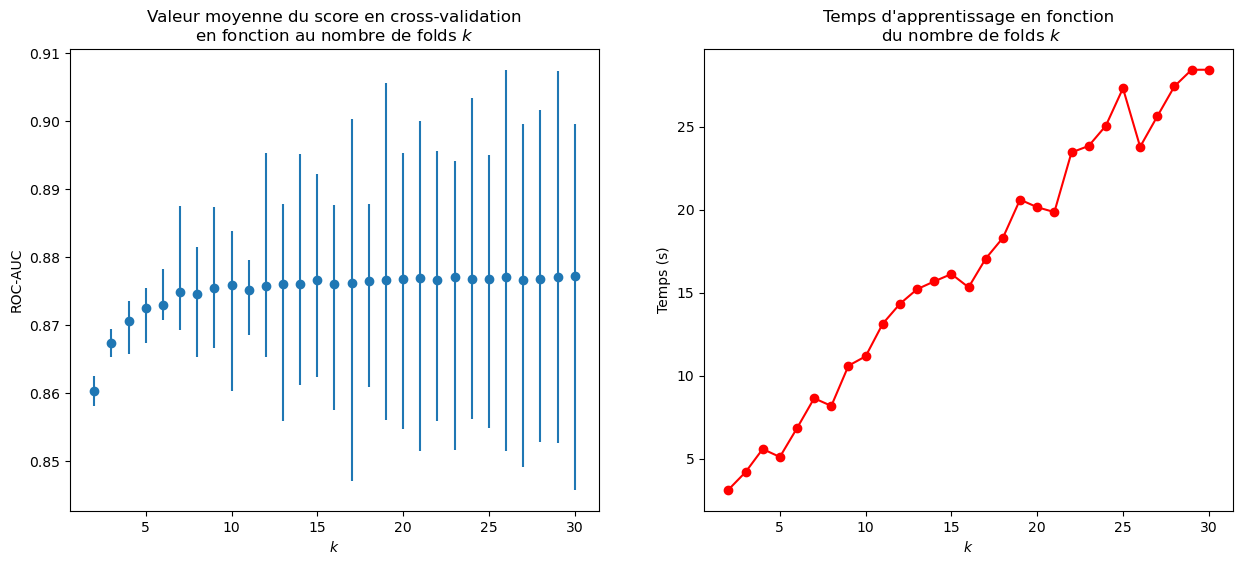
\includegraphics[width=\textwidth]{./src/locuteur/crossval_analysis.png} 
    \caption{Optimisation du nombre de folds}
    \label{crossval_analysis_pres}
\end{figure}

\subsubsection{Déséquilibre des classes}

Nous rappelons que nous avons affaire à des données très déséquilibrés : la question s'est donc posée : devons-nous rééquilibrer nos données ? Devons-nous régulariser nos données, c'est-à-dire jouer sur la fonction de coût (ajout de poids) de nos modèles ? Cela fait par l'intermédiaire du paramètre \texttt{fit\_prior} dans le cas du classifieur naïf Bayésien ou du paramètre \texttt{class\_weight} pour les deux autres modèles. On rappelle que la fonction de coût peut s'écrire de la forme (pour une classification binaire) : 
$$\text{coût} = \frac 1n \sum_{i=1}^n -w_{-1} y_i \log (\hat{y_i}) -w_1 y_i \log (\hat{y_i})$$

Dans le cas de données équilibrées, $w_{-1} = w_1$ mais dans le cas de données équilibrées, $w_{-1} > w_{1}$, ce qui pénalise mieux la classe minoritaire (-1).

Il existe différentes techniques pour rééquilibrer des données déséquilibrées en machine learning, et l'oversampling et l'undersampling en sont deux exemples courants.

L'oversampling consiste à augmenter le nombre d'instances de la classe minoritaire en créant des copies des observations existantes. Cette technique peut être utile lorsque la quantité de données est limitée, mais elle peut également entraîner un risque de surajustement si la même instance est utilisée à la fois dans l'ensemble d'apprentissage et dans l'ensemble de validation.

L'undersampling consiste à réduire le nombre d'instances de la classe majoritaire en éliminant des observations au hasard jusqu'à ce que la distribution des classes soit plus équilibrée. Cette technique peut être efficace lorsque la quantité de données est suffisamment importante, mais elle peut entraîner une perte d'information si des observations importantes sont supprimées.

Encore une fois, nous nous basons sur des modèles non paramétrés. Nous obtenons les résultats suivants : équilibrer les données change très sensiblement le score AUC obtenu, positivement dans le cadre du classifieur NB et négativement pour LogReg et SVM. Il n'a pas été possible d'obtenir les mêmes courbes pour les classes avec le SVM de fait de l'impossibilité de prédire des probabilités depuis un tel modèle, mais les résultats sont similaires au modèle de régression logistique. C'est également le cas si on se concentre uniquement sur les scores pour chacune de nos classes. C'est pourquoi nous avons décidé d'écarter de notre grille de recherche l'équilibrage des données. Enfin, nous remarquons que nous obtenons des scores plus que corrects sans avoir paramétrés notre modèle

\begin{figure}[H]
    \centering
    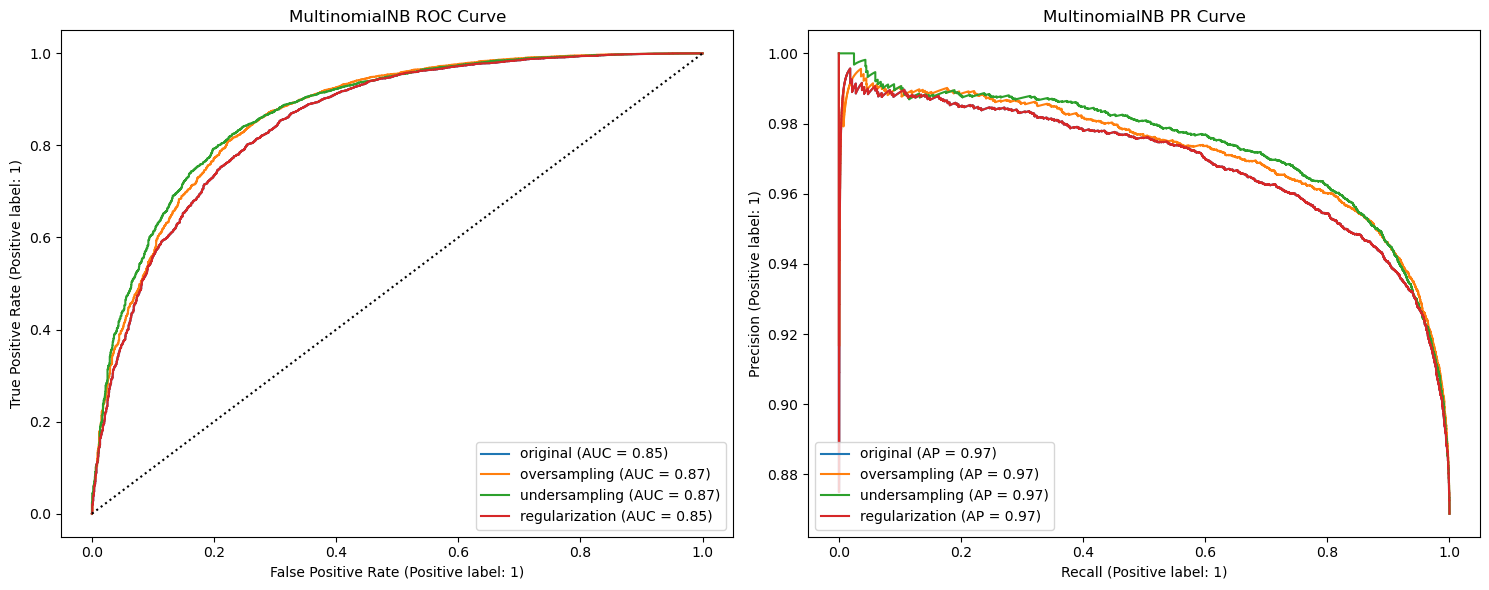
\includegraphics[width=\textwidth]{./src/locuteur/roc_curve_MultinomialNB.png} 
    \caption{Courbes ROC et Précision-Rappel en baseline, Bayésien naïf}
    \label{roc_curve_MultinomialNB}
\end{figure}

\begin{figure}[H]
    \centering
    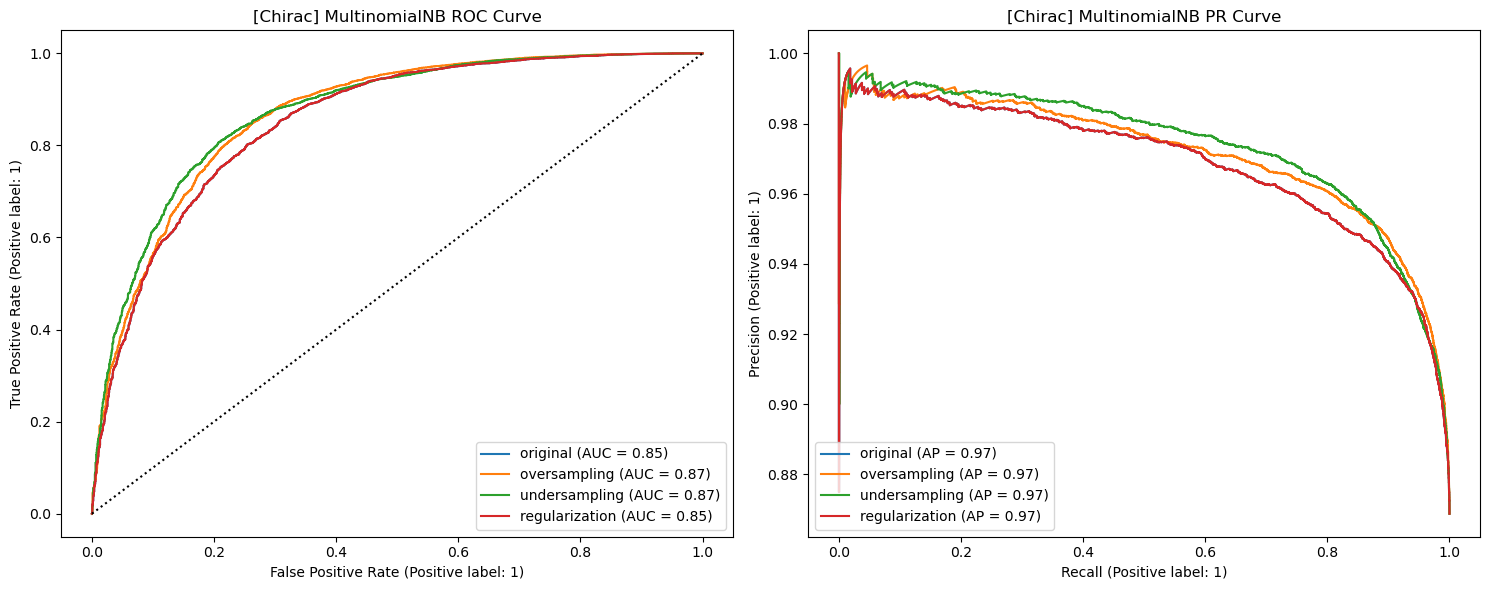
\includegraphics[width=\textwidth]{./src/locuteur/roc_curve_MultinomialNB_Chirac.png} 
    \caption{Courbes ROC et Précision-Rappel en baseline, Chirac, Bayésien naïf}
    \label{roc_curve_MultinomialNB_Chirac}
\end{figure}

\begin{figure}[H]
    \centering
    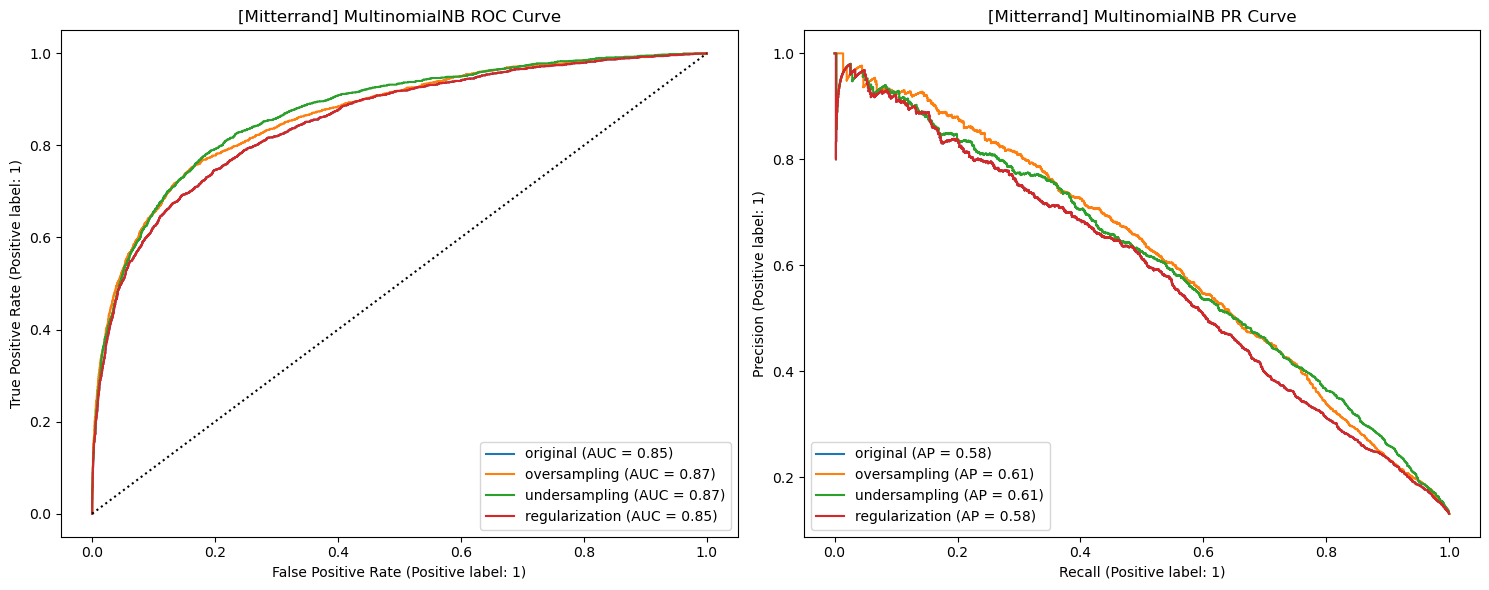
\includegraphics[width=\textwidth]{./src/locuteur/roc_curve_MultinomialNB_Mitterrand.png} 
    \caption{Courbes ROC et Précision-Rappel en baseline, Mitterrand, Bayésien naïf}
    \label{roc_curve_MultinomialNB_Mitterrand}
\end{figure}

\begin{figure}[H]
    \centering
    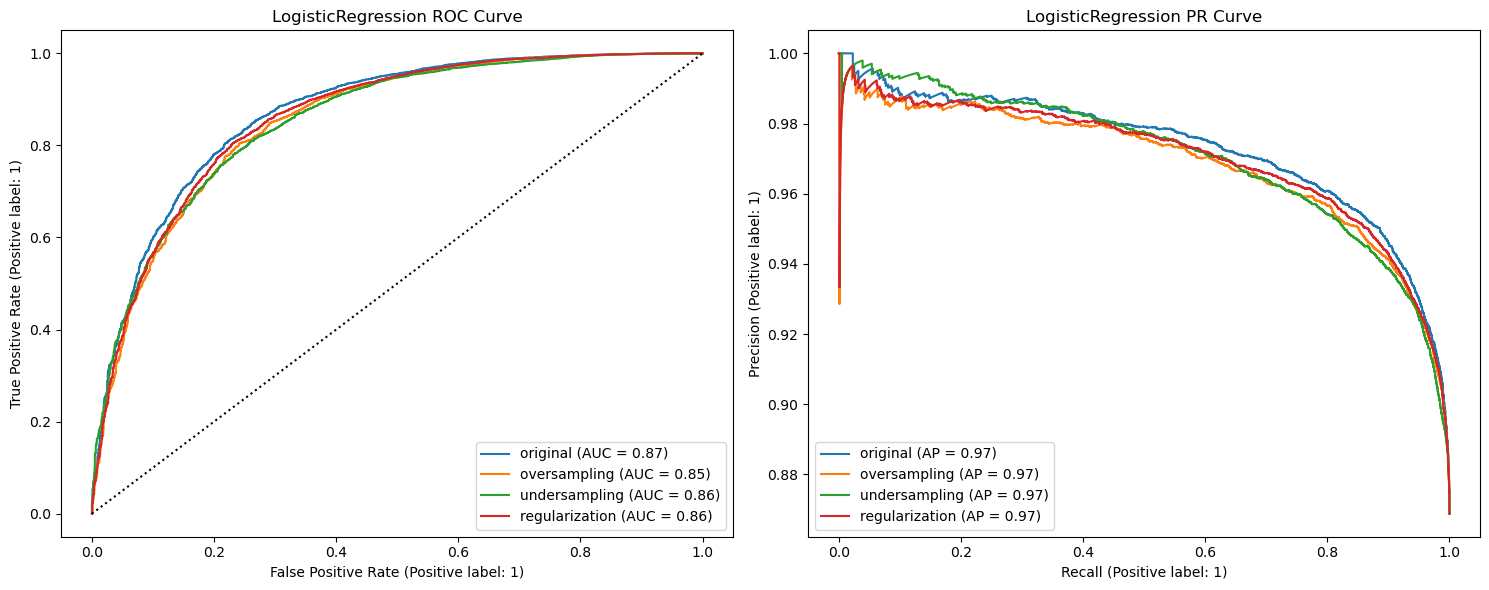
\includegraphics[width=\textwidth]{./src/locuteur/roc_curve_LogisticRegression.png} 
    \caption{Courbes ROC et Précision-Rappel en baseline, régression logistique}
    \label{roc_curve_LogisticRegression}
\end{figure}

\begin{figure}[H]
    \centering
    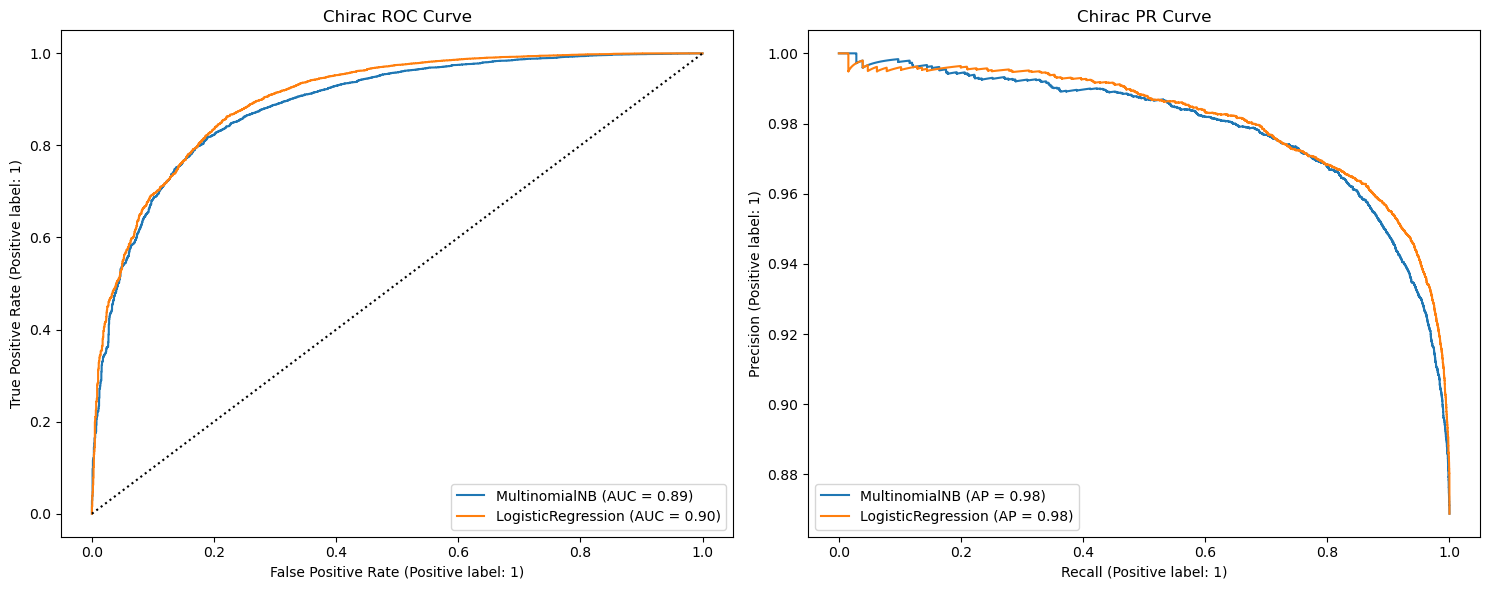
\includegraphics[width=\textwidth]{./src/locuteur/roc_curve_LogisticRegression_Chirac.png} 
    \caption{Courbes ROC et Précision-Rappel en baseline, Chirac, régression logistique}
    \label{roc_curve_LogisticRegression_Chirac}
\end{figure}

\begin{figure}[H]
    \centering
    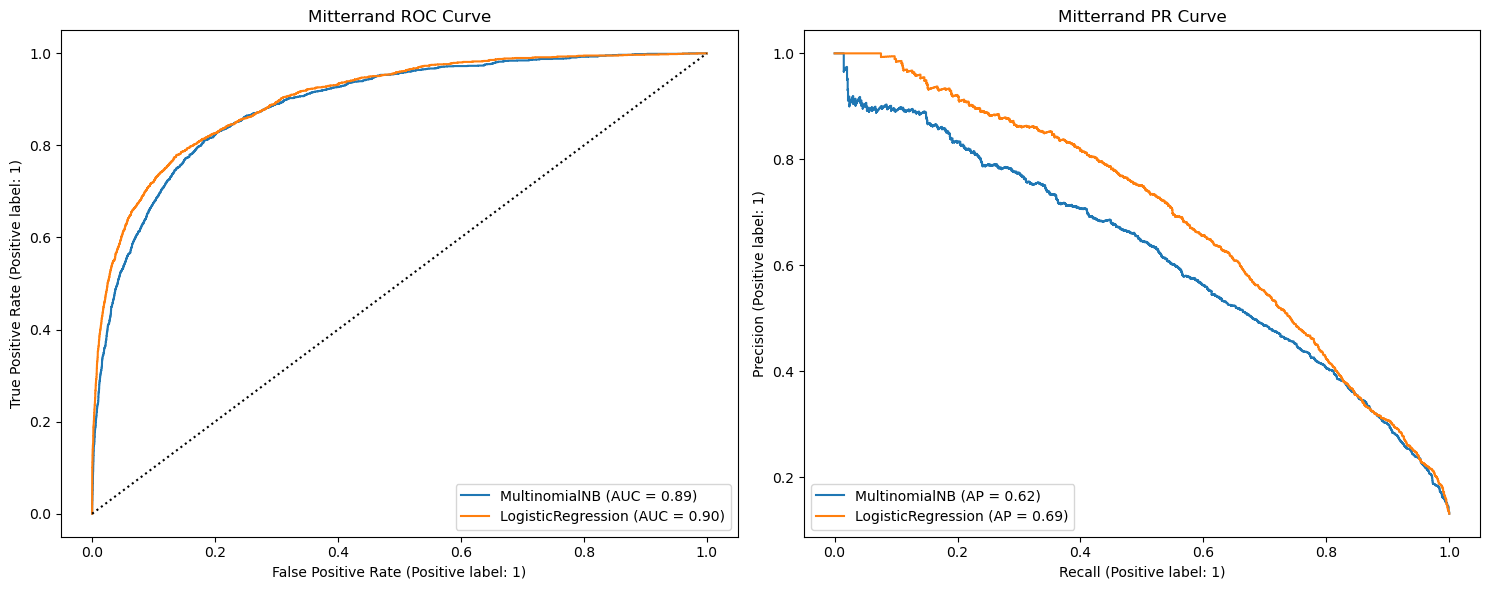
\includegraphics[width=\textwidth]{./src/locuteur/roc_curve_LogisticRegression_Mitterrand.png} 
    \caption{Courbes ROC et Précision-Rappel en baseline, Mitterrand, régression logistique}
    \label{roc_curve_LogisticRegression_Mitterrand}
\end{figure}

\begin{figure}[H]
    \centering
    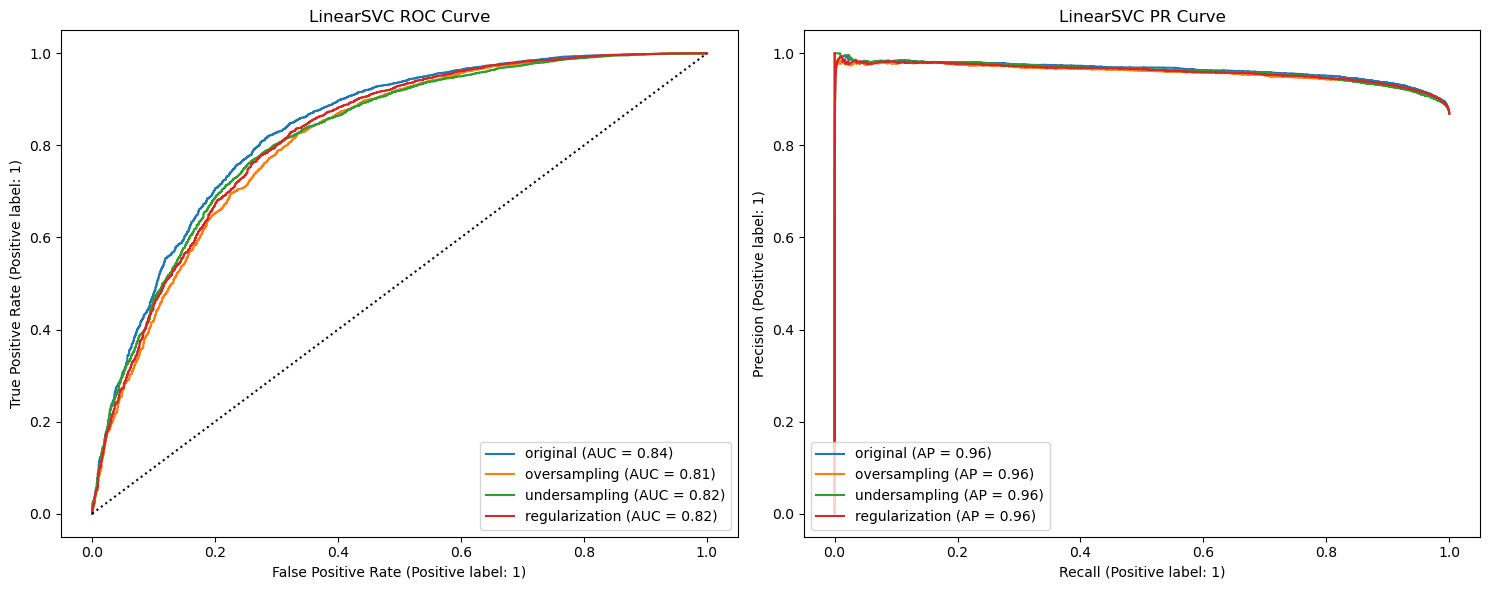
\includegraphics[width=\textwidth]{./src/locuteur/roc_curve_LinearSVC.png} 
    \caption{Courbes ROC et Précision-Rappel en baseline, SVM linéaire}
    \label{roc_curve_LinearSVC}
\end{figure}

\paragraph{Existe-t-il d'autres estimateurs pour évaluer de performance ?}

En plus des scores F1 et ROC, nous avons étudié d'autres scores pour ce projet. En effet, ce sont des scores pertinents pour les données déséquilibrées mais nous nous sommes intéressés à deux scores supplémentaires : le Kappa de Cohen et le Matthews corrélation coefficient (MCC).

Le Kappa de Cohen mesure la cohérence entre les prédictions du modèle et les vraies étiquettes, en prenant en compte la possibilité de concordance aléatoire. Il prend des valeurs entre -1 et 1, où 1 indique une concordance parfaite entre les prédictions et les étiquettes, 0 indique une concordance aléatoire et -1 indiquent une discordance totale.

Le MCC mesure la corrélation entre les prédictions du modèle et les vraies étiquettes en considérant les quatre éléments de la matrice de confusion (vrai positif, faux positif, vrai négatif, faux négatif). Le coefficient prend des valeurs entre -1 et 1, où 1 indique une concordance parfaite entre les prédictions et les étiquettes, 0 indique une concordance aléatoire et -1 indiquent une discordance totale. Le MCC est particulièrement utile pour les problèmes de classification binaire lorsque les classes sont déséquilibrées.

Pour évaluer les performances, nous l'avons également fait en évaluant uniquement le score F1 de la classe déséquilibrée (Mitterrand). Les meilleures performances ont été obtenues en mesurant les performances à l'aide du ROC-AUC et du MCC.

\subsection{Autour des blocs de discours}
Lors de l'analyse de ces phrases, et comme précisé dans le sujet, nous nous sommes rendus compte d'un point primordial à aborder dans notre analyse. Les locuteurs tendent à énoncer plusieurs phrases consécutives, ce qui permet de détecter facilement un bruit s'il est isolé. En effet, les données sont des phrases issues de discours. Mais ces phrases n'ont pas été mélangées : on retrouve des discours en entier, si l'on lit les phrases consécutivement. Ainsi, les phrases sont organisées en ce que nous avons nommé des \og blocs de discours \fg, qui ont été divisés en phrases et sont utilisés comme prédiction. Cette organisation a donné lieu à plusieurs idées, que nous détaillerons dans cette section. La première idée était de former un modèle sur l'ensemble des blocs, ce qui a conduit à d'autres possibilités. La deuxième idée était de post-traiter les prédictions obtenues pour éliminer le bruit. D'autres statistiques intéressantes sont représentées à l'aide de boxplots sur la figure \ref{boxplot_discours}. Ainsi, Chirac prononce en moyenne 124 phrases (médiane : 130, minimum : 3, maximum : 952) contre  18 phrases (médiane : 5, minimum : 3, maximum : 39) pour son homologue : de grandes différences ! Enfin, dans ce mode de réflexion, les données sont équilibrées : 401 blocs pour Chirac contre 400 pour Mitterrand.

\begin{figure}[H]
    \centering
    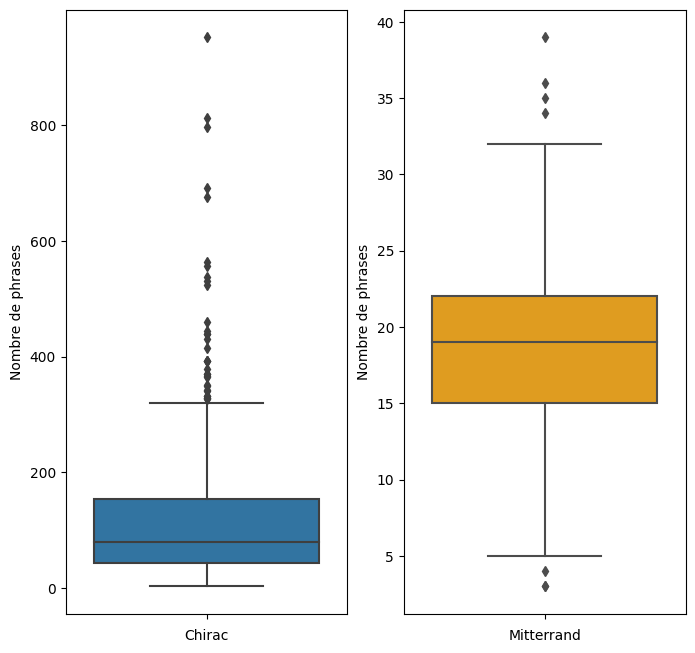
\includegraphics[width=0.6\textwidth]{./src/locuteur/boxplot_discours.png} 
    \caption{Statistiques descriptives sur les discours}
    \label{boxplot_discours}
\end{figure}

\subsubsection{Prédire des blocs de phrases}

Ainsi, la première idée fut de fonctionner par \textit{a priori} et de se dire : et si on apprenait non pas sur des phrases, mais sur ces blocs ? Comme précédemment, avant de lancer nos grandes expériences, nous avons tracé quelques courbes AUC pour évaluer le modèle et savoir quelles méthodes privilégiées. Les résultats obtenus ont confirmé notre idée d'approfondir au maximum cette idée. En effet, les performances obtenues sont parfaites (figure \ref{roc_curve_blocks} et \ref{roc_curve_blocks_classes})... Mais seulement si on effectue notre classification et notre prédiction sur des discours, et pas des phrases (figure \ref{roc_curve_blocks_phrase} et \ref{roc_curve_blocks_classes_phrase}).

\begin{figure}[H]
    \centering
    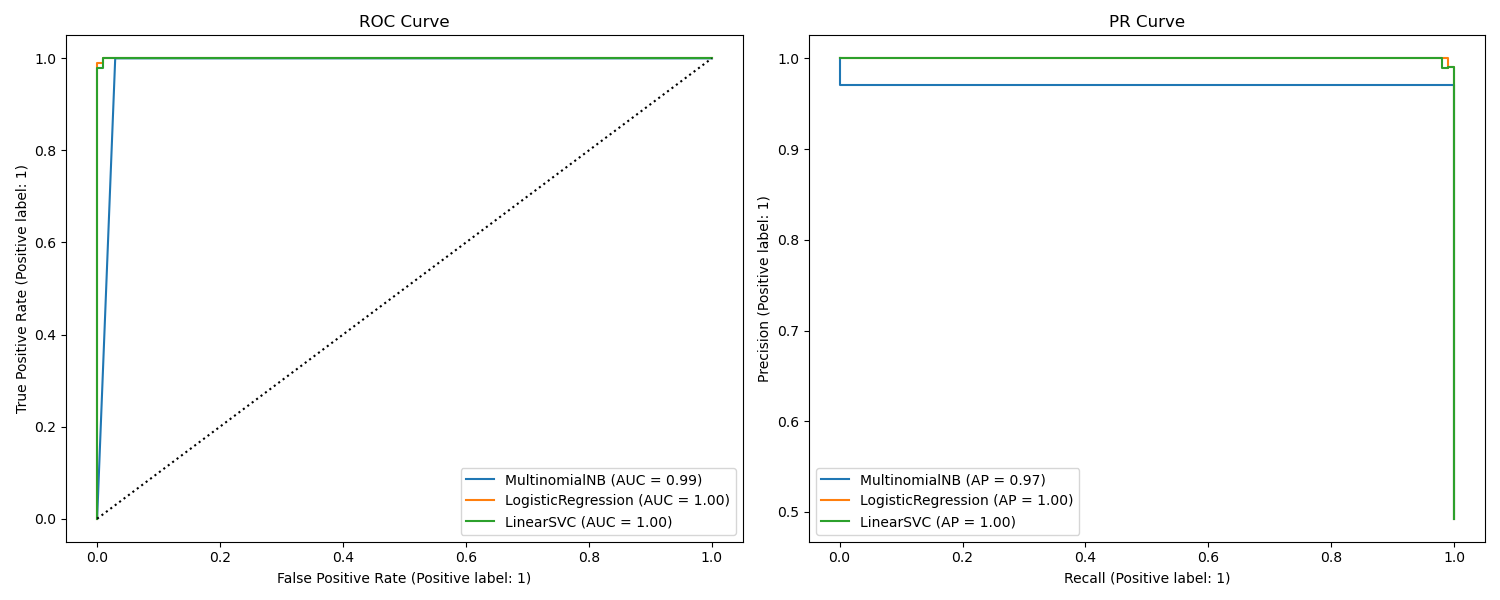
\includegraphics[width=\textwidth]{./src/locuteur/roc_curve_blocks.png} 
    \caption{Performance globale du modèle de discours, classifiant des discours}
    \label{roc_curve_blocks}
\end{figure}

\begin{figure}[H]
    \centering
    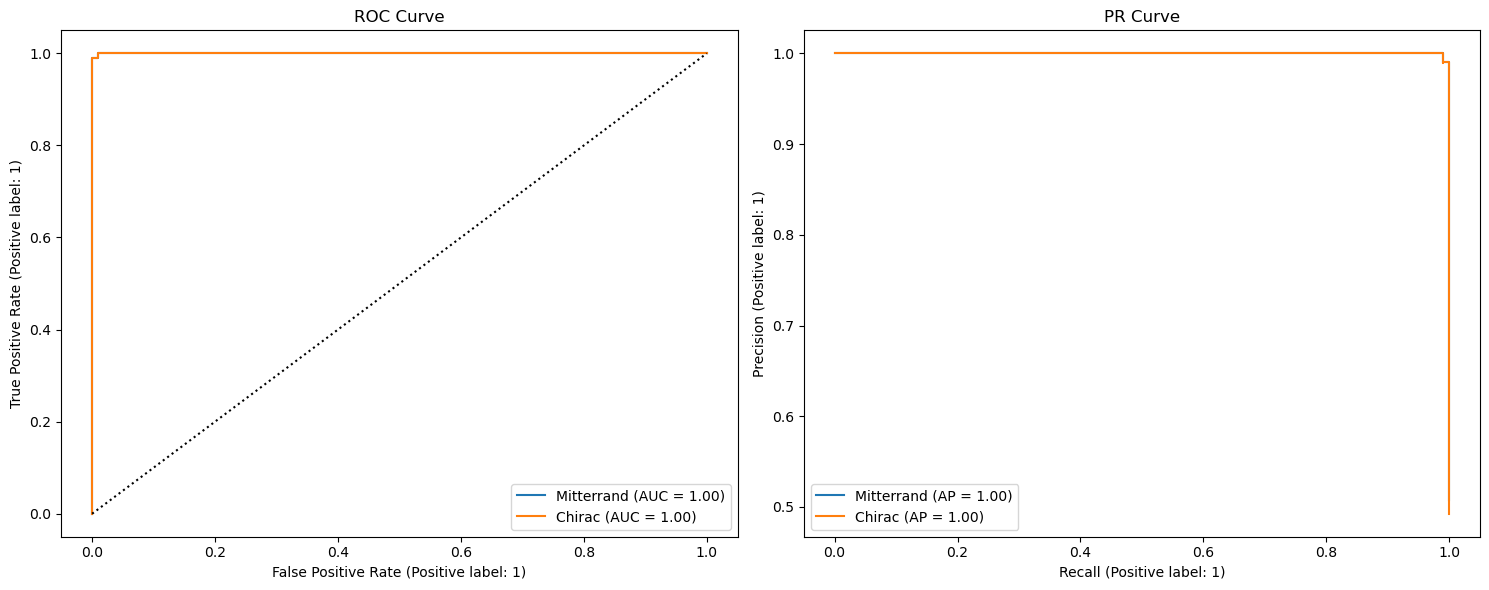
\includegraphics[width=\textwidth]{./src/locuteur/roc_curve_blocks_classes.png} 
    \caption{Performance par classe du modèle de discours, classifiant des discours}
    \label{roc_curve_blocks_classes}
\end{figure}

En effet, si on apprend sur des discours et qu'on prédit sur des phrases, les performances chutent et sont bien moindres que les modèles se basant uniquement sur les phrases ! (Figure \ref{roc_curve_blocks_phrase} et \ref{roc_curve_blocks_classes_phrase})

\begin{figure}[H]
    \centering
    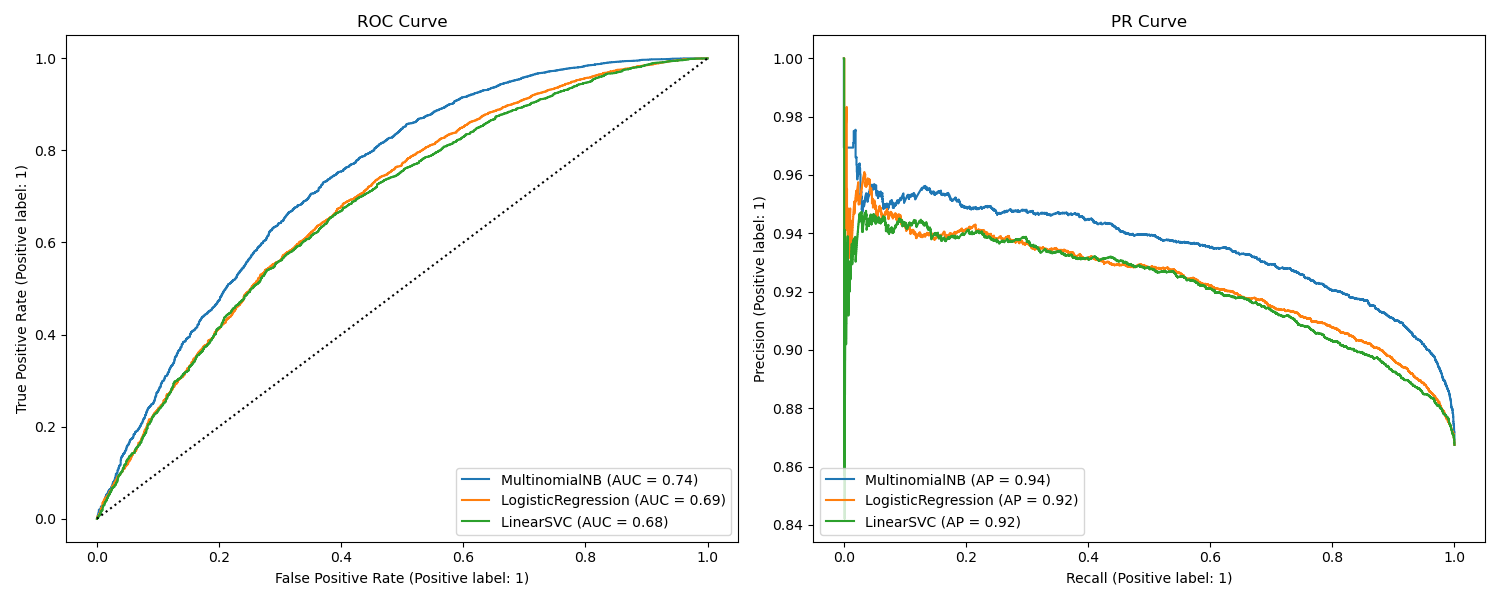
\includegraphics[width=\textwidth]{./src/locuteur/roc_curve_blocks2.png} 
    \caption{Performance globale du modèle de discours, classifiant des phrases}
    \label{roc_curve_blocks_phrase}
\end{figure}

\begin{figure}[H]
    \centering
    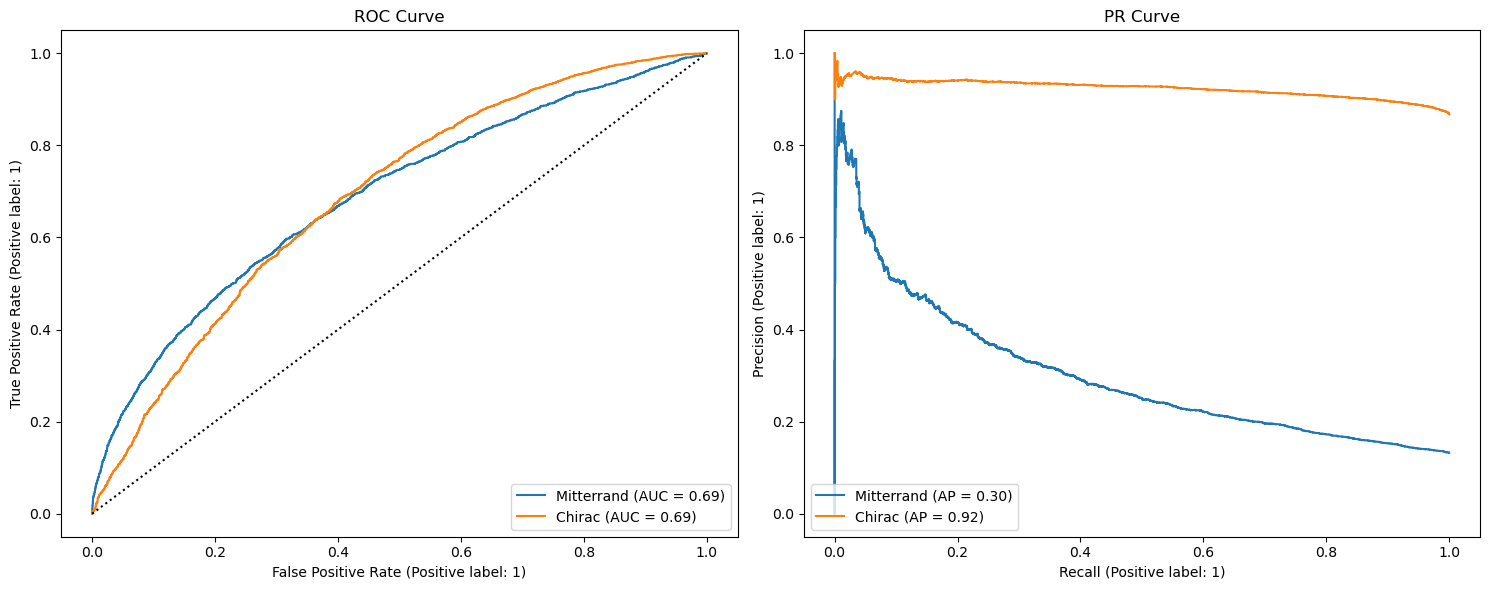
\includegraphics[width=\textwidth]{./src/locuteur/roc_curve_blocks2_classes.png} 
    \caption{Performance par classe du modèle de discours, classifiant des phrases}
    \label{roc_curve_blocks_classes_phrase}
\end{figure}

Après avoir découvert la grande performance des modèles entraînés sur les discours complets, nous avons cherché des méthodes pour reproduire ces résultats sans avoir accès aux étiquettes qui permettent la délimitation des discours. Après un rapide coup d'œil du coté des modèles séquentiels markoviens qui ne semblait pas adapté à notre cas, nous avons eu l'idée d'entraîner le modèle sur des blocs de $n$ phrases à la manière des bi-grammes ou tri-grammes.

L'entraînement se passait donc sur des blocs de $n$ phrases correctement découpés, c'est-à-dire qu'il n'y avait pas de blocs de phrases mixtes, situés à la frontière de deux discours. Puis, nous avons effectué des prédictions sur un ensemble de test, qui pouvait donc quant à lui être mal découpé, avec des blocs de phrases hybrides. Nous pensions que le gain potentiel sur la prédiction allait être supérieur à la perte engendrée par ces blocs frontières.

Les résultats sont présentés dans la figure \ref{fig_n-sentence-perf} en utilisant les scores F1 sur Mitterrand uniquement. Nous avons constaté que cette méthode faisait décroître les performances des modèles, ce qui a été une grande déception en comparaison des performances obtenues lorsque des discours complets étaient fournis en entrée.

\begin{figure}[H]
    \centering
    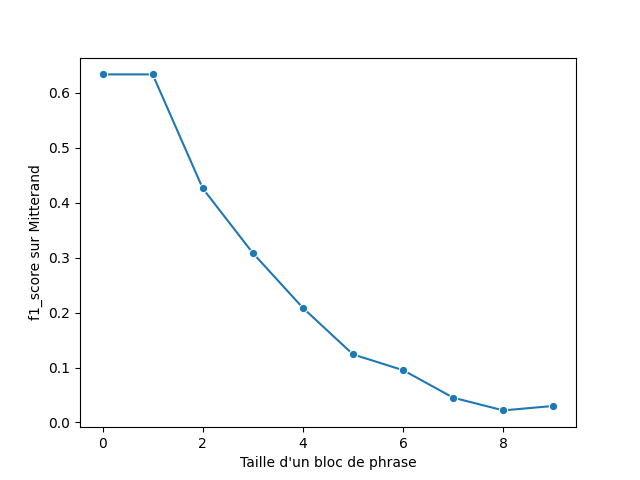
\includegraphics[width=.75\textwidth]{src/locuteur/n-sentence_bloc_perf.png}
    \caption{Impact de la taille des blocs de phrase sur le score F1 de Mitterrand}
    \label{fig_n-sentence-perf}
\end{figure}

Ces résultats ont confirmé notre hypothèse que lorsque des blocs de discours complets sont fournis, le modèle est capable de différencier les deux jeux de données par leur taille et non par leur contenu.

Néanmoins, cet \textit{a priori} sur les données n'est pas à écarter, au vu des résultats que nous avons obtenus. Mais si, au lieu de fonctionner par \textit{a priori}, nous fonctionnons par \textit{a posteriori} ? C'est de ce constat que nous est venue l'idée du \textit{post-processing}, que nous allons maintenant présenter.



\subsubsection{Post-traitement}

Le post-traitement consistait à détecter les prédictions de type "bruit" et à les corriger, ce qui a permis d'améliorer considérablement les deux scores proposés sur la plateforme de généralisation. Par exemple, une phrase attribuée à Mitterrand, entourée de dix phrases attribuées à Chirac, est très probablement une mauvaise classification dans un bloc de discours de Chirac, d'où cette qualification de "bruit". 

L'idée était donc de faire passer une fenêtre sur la liste des prédictions, à la manière d'un noyau de convolution, de compter le nombre de points de chaque classe, et d'attribuer la classe la plus fréquente au point sur lequel la fenêtre était centrée. Le paramètre décisif était la taille du noyau, c'est-à-dire le nombre de voisins à prendre en compte pour déterminer si le point était un bruit ou non.

Trois expériences ont été menées :
\begin{enumerate}
    \item Impact de la taille de la fenêtre ; \label{bloc_exp_1}
    \item Passage multiple d'une fenêtre de taille fixe ; \label{bloc_exp_2}
    \item Passage multiple d'une fenêtre de taille croissante. \label{bloc_exp_3}
\end{enumerate}

La figure \ref{fig_bloc_exp} illustre les résultats des expériences \ref{bloc_exp_1} et \ref{bloc_exp_3}. L'axe des ordonnées représente le score F1, calculé uniquement pour la classe minoritaire de Mitterrand ($-1$), tandis que l'axe des abscisses représente la taille de la fenêtre. Une fenêtre de taille zéro correspondait à la ligne de base. Nous avons constaté une efficacité notable de cette méthode, avec un score de ligne de base de $0.55$ qui est passé à $0.77$.

\begin{figure}[H]
    \centering
    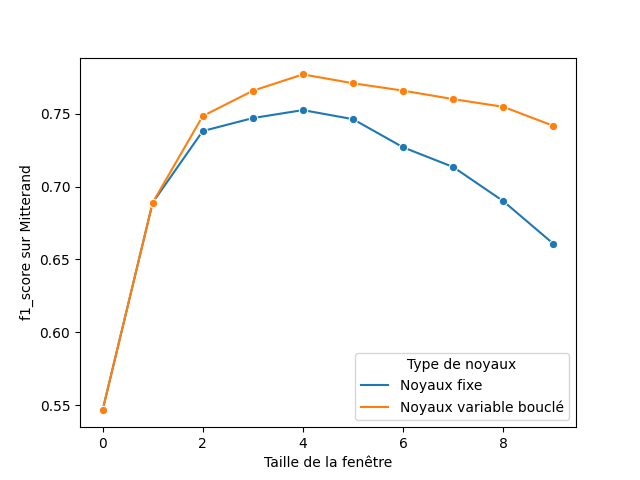
\includegraphics[width=.75\textwidth]{src/locuteur/kernel_type_impact.png}
    \caption{Impact de la taille de la fenêtre sur le f1-score de Mitterrand}
    \label{fig_bloc_exp}
\end{figure}

L'expérience \ref{bloc_exp_2} a montré qu'il n'y avait pas d'impact significatif à passer plusieurs fois une fenêtre de taille fixe (score constant).

Afin de mieux comprendre l'efficacité remarquable de cette méthode, nous avons examiné les matrices de confusion. Nous avons observé que le post-traitement transformait globalement les prédictions de classe $-1$ en classe $1$ pour la classe $1$ (figure \ref{fig:two_confusion_matrix}. Ainsi, un modèle qui prédit beaucoup plus de classe $-1$ que de classe $1$, mais qui est plus précis lorsque le vrai label est de classe $-1$, sera mieux corrigé par le post-traitement. En ce faisant, on améliore le score pour chacune des classes : beaucoup de Chirac mal classé se retrouve bien classé, augmentant donc le recall pour cette classe et entraine par la même occasion une amélioration de la précision pour Mitterrand. C'est ainsi que nous avons obtenu nos meilleurs résultats sur l'ensemble de validation, avec un score F1 de $0.82$ et une AUC de $0.86$.


\begin{figure}[htbp]
  \centering
  \begin{subfigure}[b]{0.45\textwidth}
    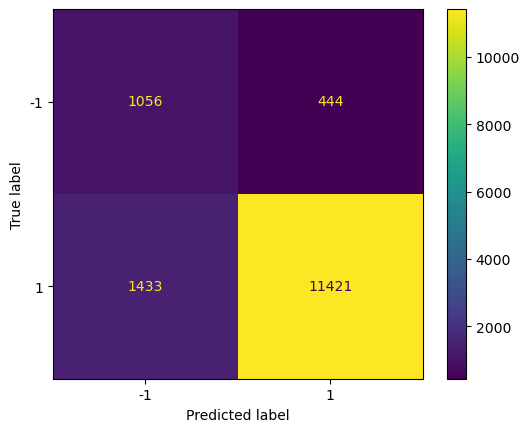
\includegraphics[width=\textwidth]{src/locuteur/confusion_matrix_no_post.png}
    \caption{Avant post-traitement}
    \label{fig:image1}
  \end{subfigure}
  \begin{subfigure}[b]{0.45\textwidth}
    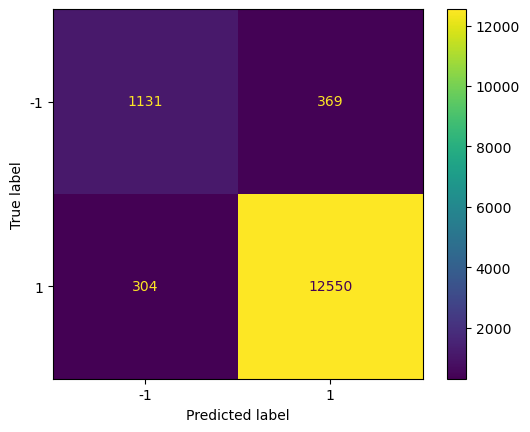
\includegraphics[width=\textwidth]{src/locuteur/confusion_matrix_with_post.png}
    \caption{Après post-traitement}
    \label{fig:image2}
  \end{subfigure}
  \caption{Matrice de confusion illustrant l'effet du post-traitement pour la régression logistique MCC}
  \label{fig:two_confusion_matrix}
\end{figure}


\subsection{Résultats et discussions}
Notre intuition, d'après les résultats précédents, est que le meilleur classifieur sera soit une régression logistique ou un SVM linéaire, avec des poids régularisés. La meilleure représentation serait un sac de mots utilisant des $n$-grammes sous une représentation TF-IDF.

Le meilleur modèle est obtenu après post-processing avec une régression logistique optimisée par MCC. Les paramètres sont listés dans la table \ref{table:MCC_pipeline}, nous avons obtenu nos meilleurs résultats sur l'ensemble de validation avec ce modèle, avec un score F1 de $0.82$ et une AUC de $0.86$. Les résultats détaillés sont disponibles dans les tables \ref{table:MMC_no_post} et \ref{table:MMC_with_post}. 

\begin{table}[H]
    \centering
    \begin{tabular}{ll}
        Paramètres & Valeurs \\ \hline
        CountVectorizer & binary=True, lowercase=False, max\_features=150000,  \\ 
        ~ & ngram\_range=(1, 3), strip\_accents='unicode' \\ 
        TfidfTransformer & smooth\_idf=False, use\_idf=False \\ 
        LogisticRegression & C=4.030086627072631, class\_weight='balanced', solver='liblinear' \\ 
    \end{tabular}
    \caption{Paramètre de la pipeline pour la régression logistique MCC}
    \label{table:MCC_pipeline}
\end{table}

Ici, un bag of words binaire est utilisé et des tuples (unigramme, bigramme, trigramme) sont utilisés pour la représentation sac de mots (en limitant la taille de notre vocabulaire à 150~000). Contrairement à notre estimation, les mots ne sont pas pondérés par TF-IDF.

\begin{table}[H]
    \centering
    \begin{tabular}{lllll}
        precision & recall & f1-score & support & ~ \\ \hline
        -1 & 0.42 & 0.70 & 0.53 & 1500 \\ 
        1 & 0.96 & 0.89 & 0.92 & 12854 \\ 
        accuracy & 0.87 & 14354 & ~ & ~ \\ 
        macro avg & 0.69 & 0.80 & 0.73 & 14354 \\ 
        weighted avg & 0.91 & 0.87 & 0.88 & 14354 \\ 
    \end{tabular}
    \caption{Résultat détaillé avant post-traitement pour la régression logistique MCC}
    \label{table:MMC_no_post}
\end{table}

\begin{table}[H]
    \centering
    \begin{tabular}{lllll}
        ~ & precision & recall & f1-score & support \\ \hline
        -1 & 0.79 & 0.75 & 0.77 & 1500 \\ 
        1 & 0.97 & 0.98 & 0.97 & 12854 \\ 
        accuracy & ~ & ~ & 0.95 & 14354 \\ 
        macro avg & 0.88 & 0.87 & 0.87 & 14354 \\ 
        weighted avg & 0.95 & 0.95 & 0.95 & 14354 \\ 
    \end{tabular}
    \caption{Résultat détaillé après post-traitement pour la régression logistique MCC}
    \label{table:MMC_with_post}
\end{table}

Enfin, on s'intéresse aux features les plus importantes de notre modèle :

\begin{figure}[H]
    \centering
    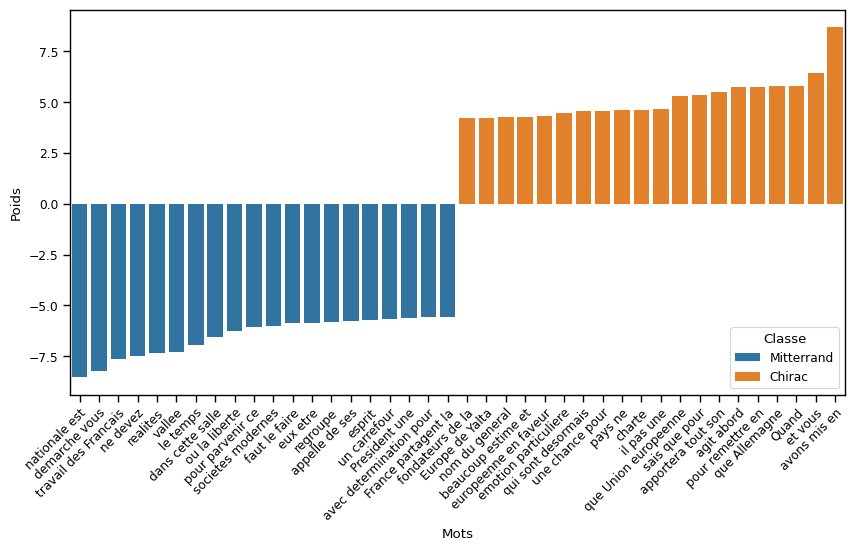
\includegraphics[width=\textwidth]{./src/locuteur/param_analysis_MCC.png}
    \caption{Top features, régression logistique}
    \label{features_logreg_mcc}
\end{figure}

Quant au meilleur modèle sans post-traitement, il est attribué à un SVM linéaire optimisé sur ROC-AUC, avec les paramètres listés dans la table \ref{table:SVC_pipeline} et les résultats dans la table \ref{table:SVC}. Ce qui surprend, c'est le faible rendement du post-traitement sur ces données contrairement au modèle précédent : le SVM classifie mieux Mitterrand, mais il créé plus de bruit.

\begin{table}[H]
    \centering
    \begin{tabular}{ll}
        Paramètres & Valeurs \\ \hline
        CountVectorizer & binary=True, lowercase=False, max\_features=500000, ngram\_range=(1, 3) \\ 
        TfidfTransformer & ~ \\ 
        LinearSVC & C=63730.28749826174, class\_weight='balanced' \\ 
    \end{tabular}
    \caption{Paramètre de la pipeline pour la Linear SVC}
    \label{table:SVC_pipeline}
\end{table}

Ici aussi, des tri-grammes utilisés mais contrairement à précédemment, une pondération TF-IDF a été effectué. 

\begin{table}[H]
    \centering
    \begin{tabular}{lllll}
        ~ & precision & recall & f1-score & support \\ \hline
        -1 & 0.56 & 0.70 & 0.62 & 1500 \\ 
        1 & 0.96 & 0.94 & 0.95 & 12854 \\ 
        accuracy & ~ & ~ & 0.91 & 14354 \\ 
        macro avg & 0.76 & 0.82 & 0.79 & 14354 \\ 
        weighted avg & 0.92 & 0.91 & 0.92 & 14354 \\ 
    \end{tabular}
    \caption{Résultat détaillé sans pour la Linear SVC}
    \label{table:SVC}
\end{table}

On se réintéresse aux features de notre modèle :

\begin{figure}[H]
    \centering
    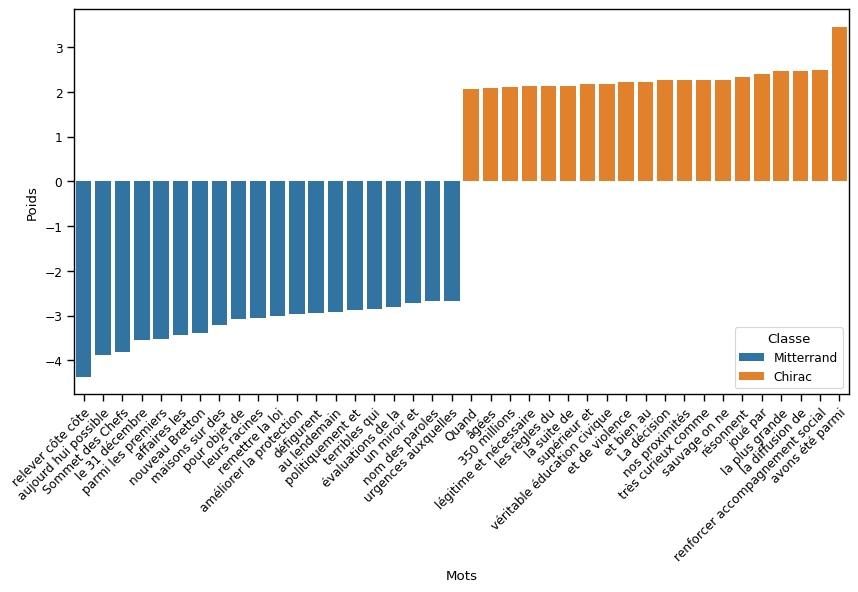
\includegraphics[width=\textwidth]{./src/locuteur/param_analysis_SVC.png}
    \caption{Top features, SVM linéaire}
    \label{features_svm}
\end{figure}


On peut voir que la régression logistique accorde plus d'intérêt au mot "Quand" que le SVM.






\section{Analyse de sentiments}

Les parties sont similaires à la partie précédente, nous commenterons donc moins les analyses mais toujours les résultats.

\subsection{Données}

Les données sont composées de 1~000 avis positifs et 1~000 avis négatifs. Ici, les données sont parfaitement équilibrées mais nous n'avons pas une quantité très grande à notre disposition. Cependant, contrairement au jeu de données précédemment, nous avons affaire à des paragraphes et non des phrases, et donc un vocabulaire plus important. Ainsi, avec stopwords, il y a 39~659 mots pour au total 1~259~869 (soit autant que les locuteurs, avec 30 fois moins de données).

\begin{figure}[H]
    \centering
    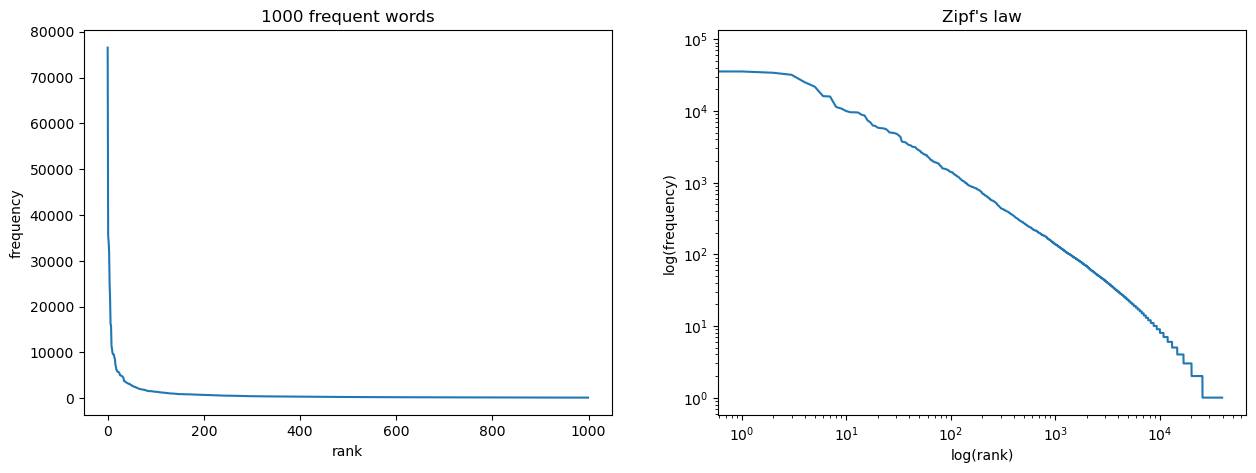
\includegraphics[width=\textwidth]{./src/movies/zipfs_nostopwords.png}
    \caption{Vocabulaire, avec stopwords}
    \label{zipfs_nostopwords_movies}
\end{figure}

\begin{figure}[H]
    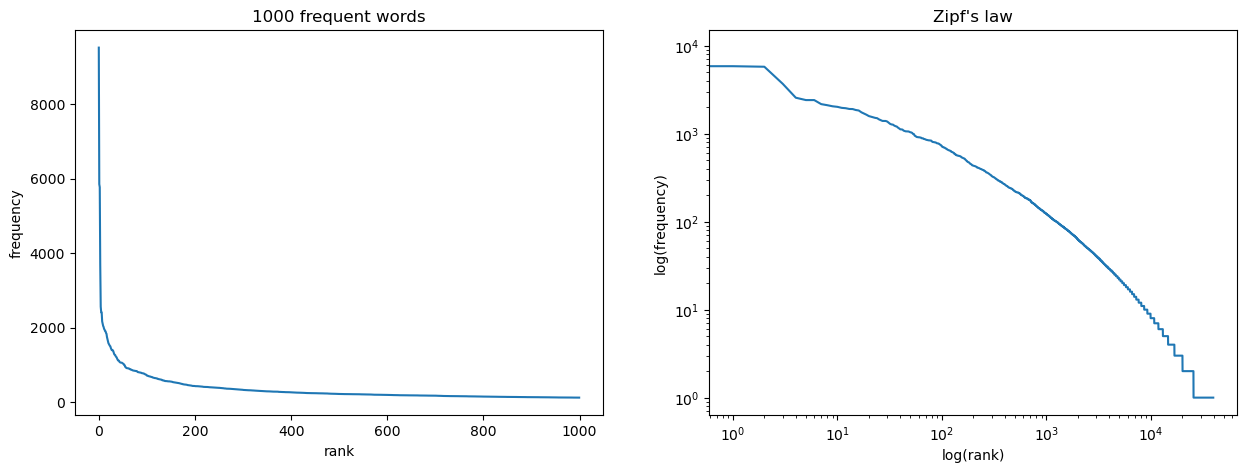
\includegraphics[width=\textwidth]{./src/movies/zipfs_stopwords.png} 
    \caption{Vocabulaire, sans stopwords}
    \label{zipfs_stopwords_movies}
\end{figure}

\begin{figure}[H]
    \centering
    \begin{minipage}[b]{0.48\textwidth}
        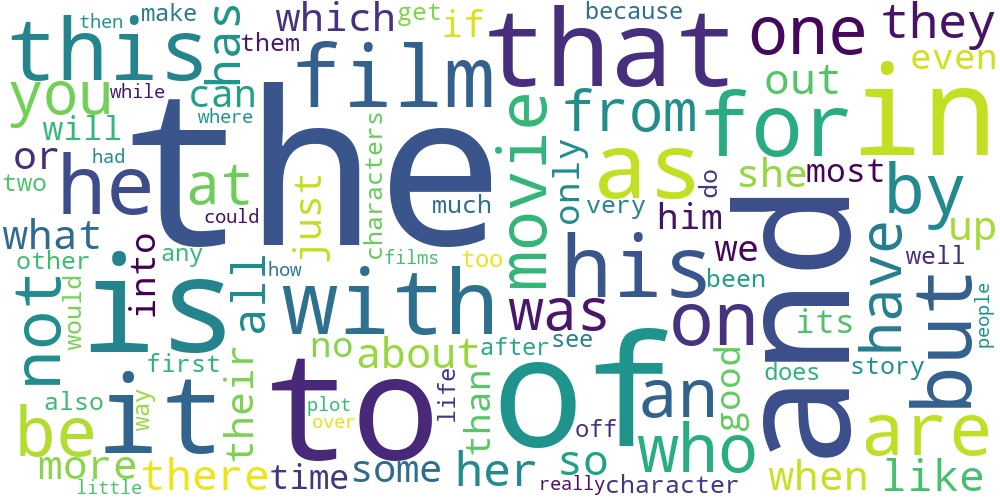
\includegraphics[width=\textwidth]{./src/movies/wordclouds_nostopwords.png}
        \caption{Nuage de mots (top 100), avec stopwords}
        \label{wordcloud_nostopwords_movies}
    \end{minipage}
    \hfill
    \begin{minipage}[b]{0.48\textwidth}
        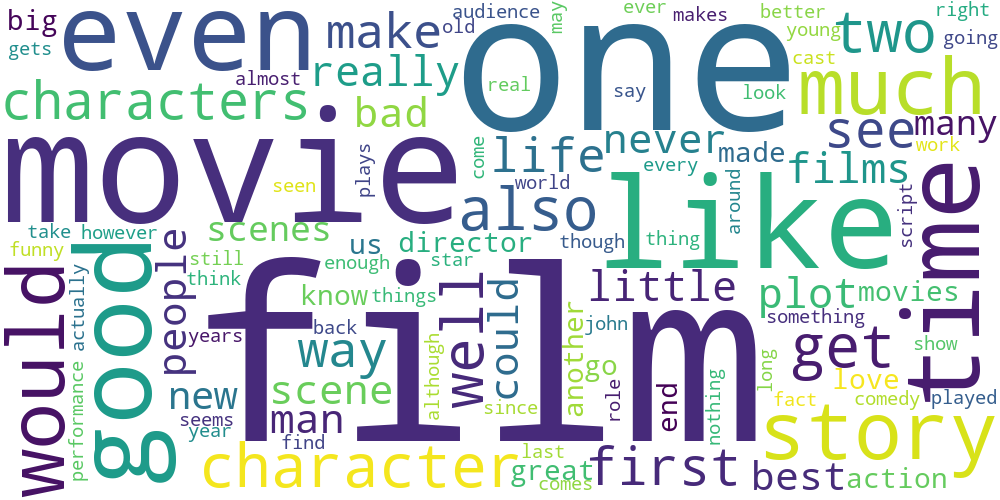
\includegraphics[width=\textwidth]{./src/movies/wordclouds_stopwords.png}
        \caption{Nuage de mots (top 100), sans stopwords}
        \label{wordcloud_stopwords_movies}
    \end{minipage}
\end{figure}

Sans les stopwords, nous avons un vocabulaire qui passe à 39~516 mots pour 705~191 au total.

\begin{figure}[H]
    \centering
    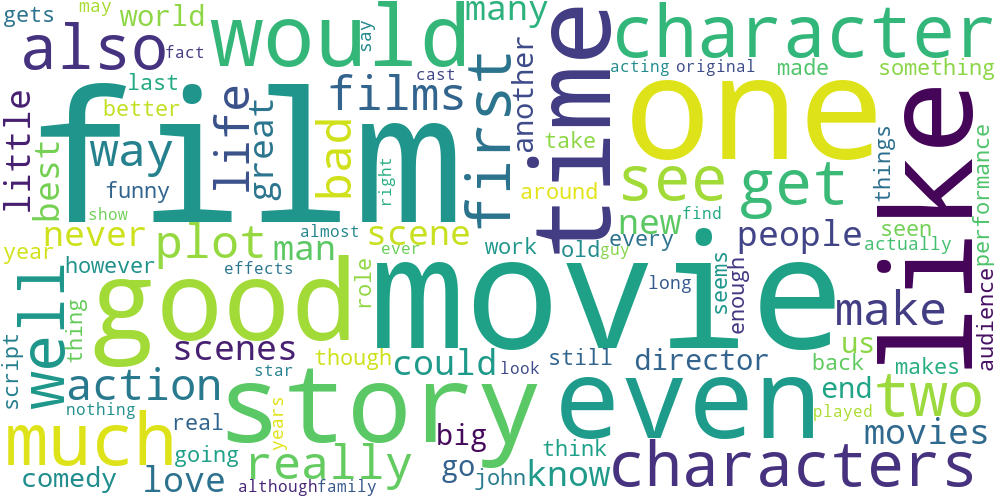
\includegraphics[width=\textwidth]{./src/movies/wordclouds_stopwords_tfidf.png}
    \caption{Nuage de mots (top 100), TF-IDF, sans stopwords}
    \label{wordcloud_stopwords_tf_idf_movies}
\end{figure}



\paragraph{Par classes}
Il est également important de regarder le vocabulaire utilisé pour chacune de nos classes, qui nous permettrait d'identifier potentiellement des mots significatifs pour la construction des poids du modèle.

\begin{figure}[H]
    \centering
    \begin{minipage}{0.48\textwidth}
        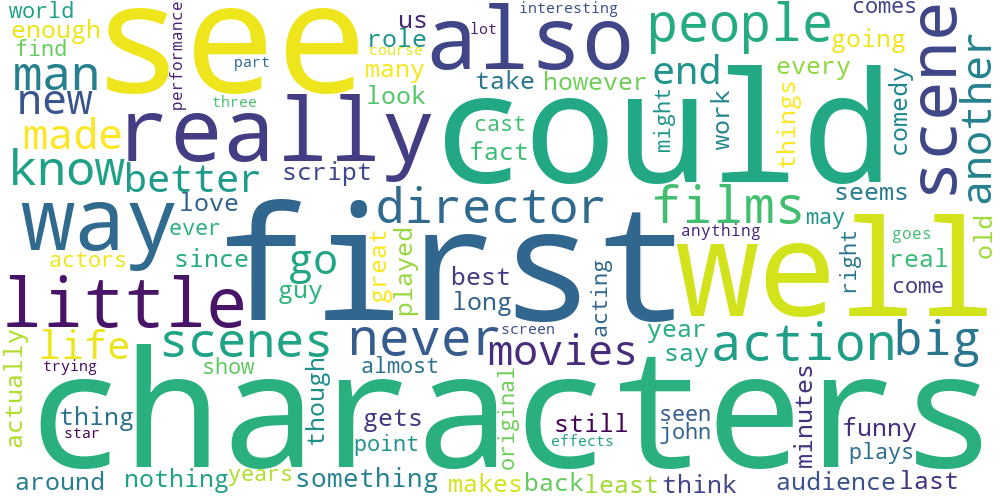
\includegraphics[width=\textwidth]{./src/movies/wordclouds_neg_nostopwords.png} 
        \caption{Nuage de mots (top 100), avis négatifs, sans stopwords}
        \label{wordclouds_neg_nostopwords}
    \end{minipage}
    \hfill
    \begin{minipage}{0.48\textwidth}
        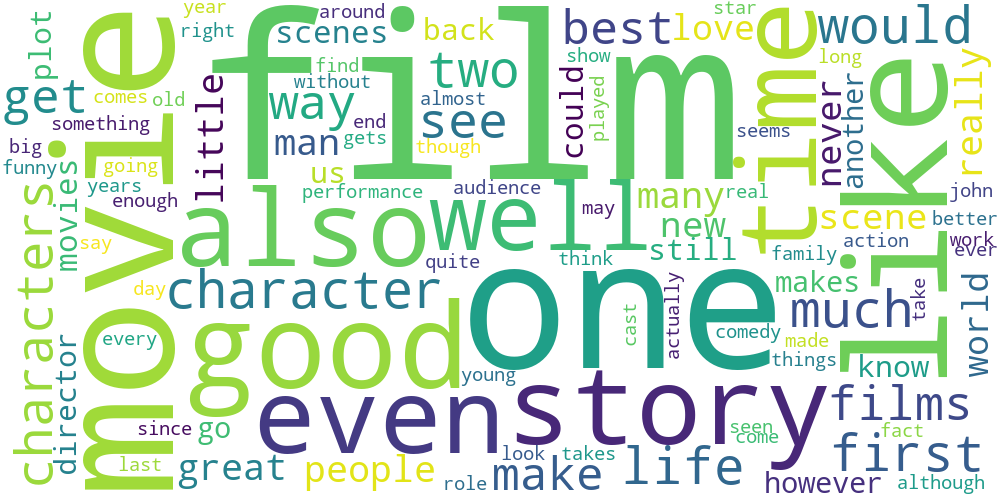
\includegraphics[width=\textwidth]{./src/movies/wordclouds_pos_nostopwords.png} 
        \caption{Nuage de mots (top 100), avis positifs, sans stopwords}
        \label{wordclouds_pos_nostopwords}
    \end{minipage}
\end{figure}

\begin{figure}[H]
    \centering
    \begin{minipage}{0.48\textwidth}
        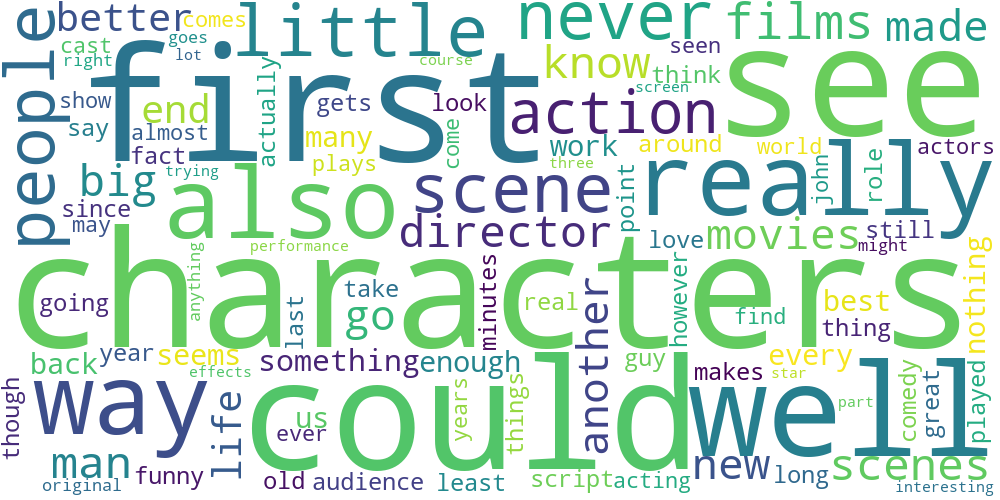
\includegraphics[width=\textwidth]{./src/movies/wordclouds_neg_stopwords_tfidf.png} 
        \caption{Nuage de mots (top 100), TF-IDF, avis négatifs, sans stopwords}
        \label{wordclouds_neg_stopwords_tfidf}
    \end{minipage}
    \hfill
    \begin{minipage}{0.48\textwidth}
        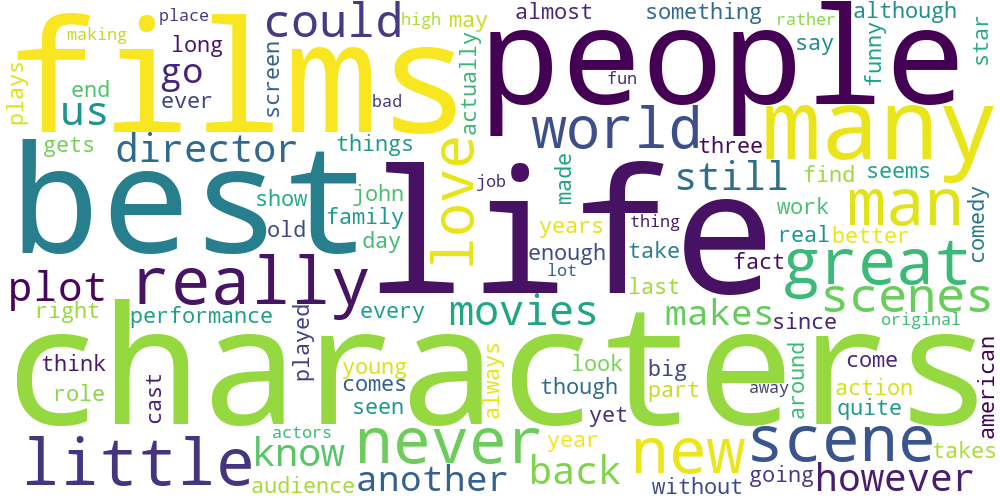
\includegraphics[width=\textwidth]{./src/movies/wordclouds_pos_stopwords_tfidf.png} 
        \caption{Nuage de mots (top 100), TF-IDF, avis positifs, sans stopwords}
        \label{wordclouds_pos_stopwords_tfidf}
    \end{minipage}
\end{figure}

\begin{figure}[H]
    \centering
    \begin{minipage}{0.48\textwidth}
        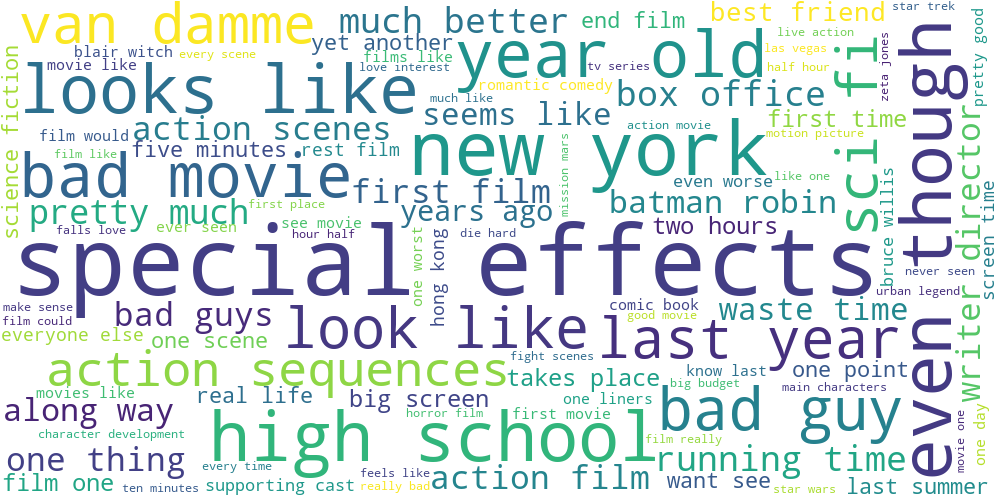
\includegraphics[width=\textwidth]{./src/movies/wordclouds_neg_nostopwords_2grams.png} 
        \caption{Nuage de mots (top 100), bigrammes, avis négatifs, sans stopwords}
        \label{fig:neg_bigrams}
    \end{minipage}
    \hfill
    \begin{minipage}{0.48\textwidth}
        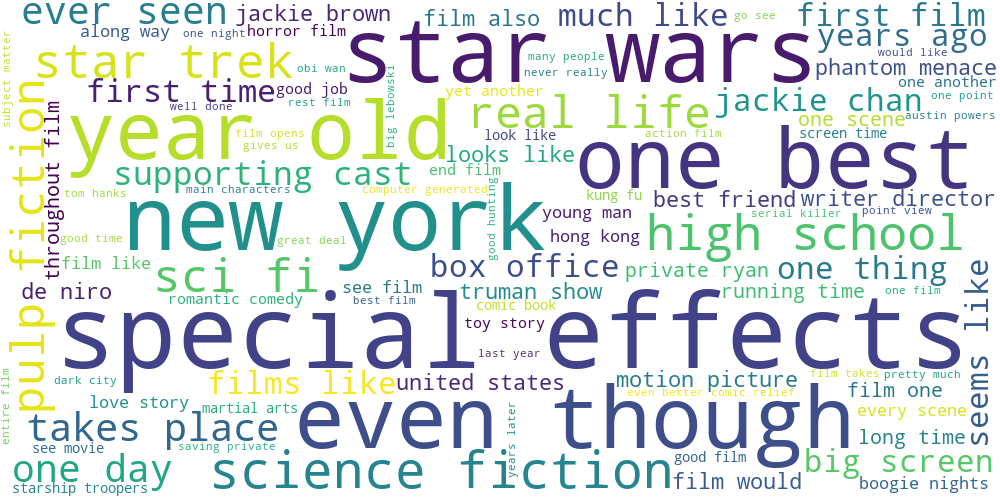
\includegraphics[width=\textwidth]{./src/movies/wordclouds_pos_nostopwords_2grams.png} 
        \caption{Nuage de mots (top 100), bigrammes, avis positifs, sans stopwords}
        \label{fig:pos_bigrams}
    \end{minipage}
\end{figure}


\begin{figure}[H]
    \centering
    \begin{minipage}{0.48\textwidth}
        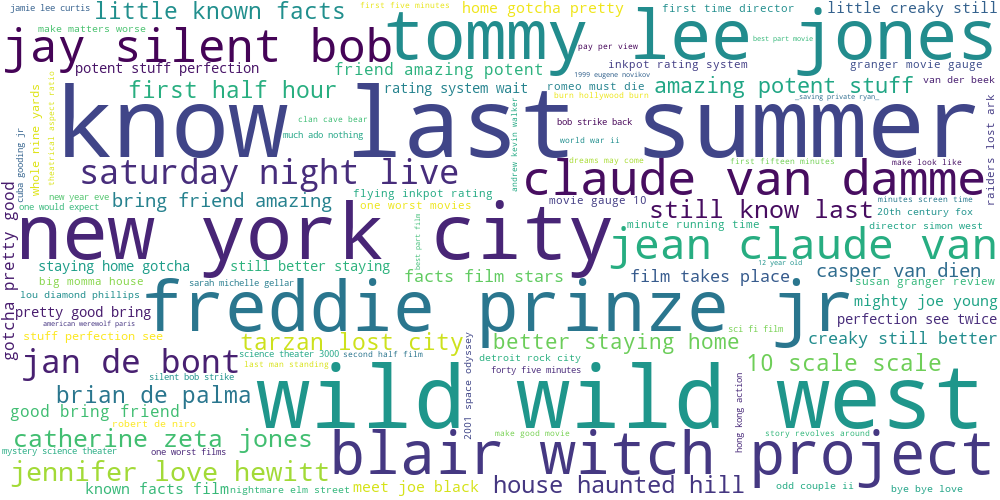
\includegraphics[width=\textwidth]{./src/movies/wordclouds_neg_nostopwords_3grams.png} 
        \caption{Nuage de mots (top 100), trigrammes, avis négatifs, sans stopwords}
        \label{wordclouds_neg_nostopwords_2grams}
    \end{minipage}
    \hfill
    \begin{minipage}{0.48\textwidth}
        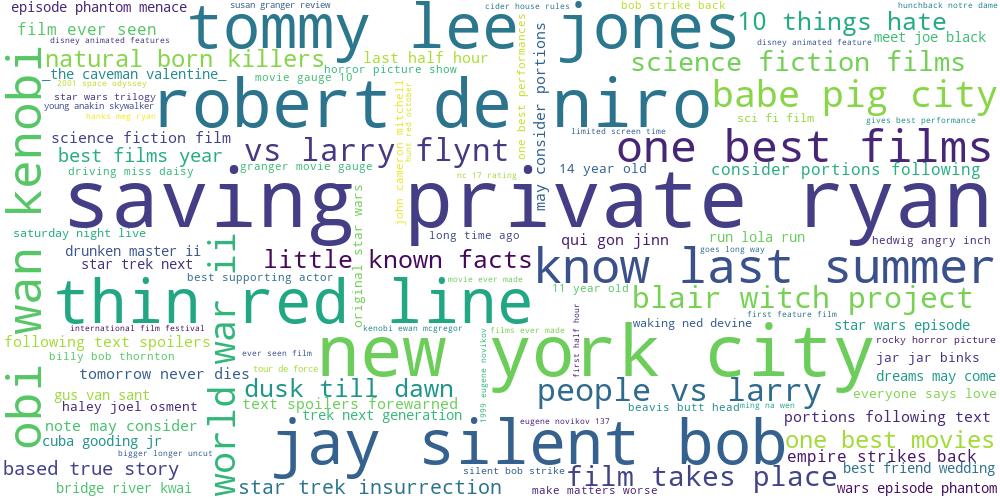
\includegraphics[width=\textwidth]{./src/movies/wordclouds_pos_nostopwords_3grams.png} 
        \caption{Nuage de mots (top 100), trigrammes, avis positifs, sans stopwords}
        \label{wordclouds_pos_nostopwords_2grams}
    \end{minipage}
\end{figure}

Certains mots redondants pour chacune des classes disparaissent en utilisant une pondération TF-IDF ou des $n$grammes. On identifie même des noms de films.

\subsection{Estimations}

De part le faible nombre de données à notre disposition, il nous est nécessaire d'avoir plus d'avoir au moins 50 \% de données d'entrainement, comme nous l'indique les courbes d'apprentissage. Nous obtenons des résultats similaires à précédemment. 

\begin{figure}[H]
    \centering
    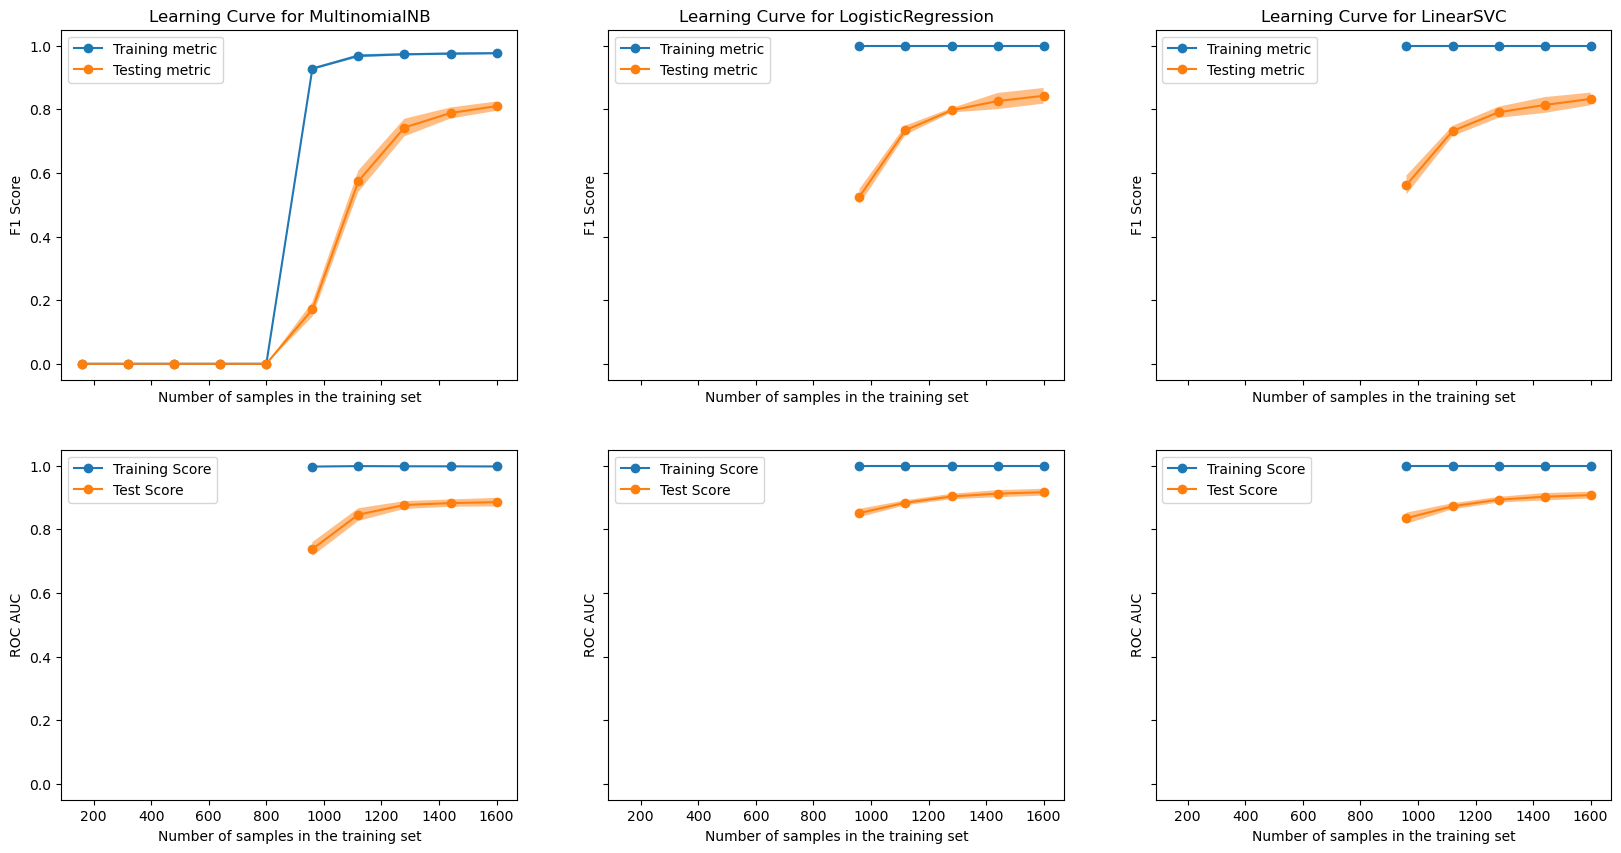
\includegraphics[width=\textwidth]{./src/movies/learningcurve.png} 
    \caption{Courbes d'apprentissage}
    \label{learningcurve_movies}
\end{figure}

\begin{figure}[H]
    \centering
    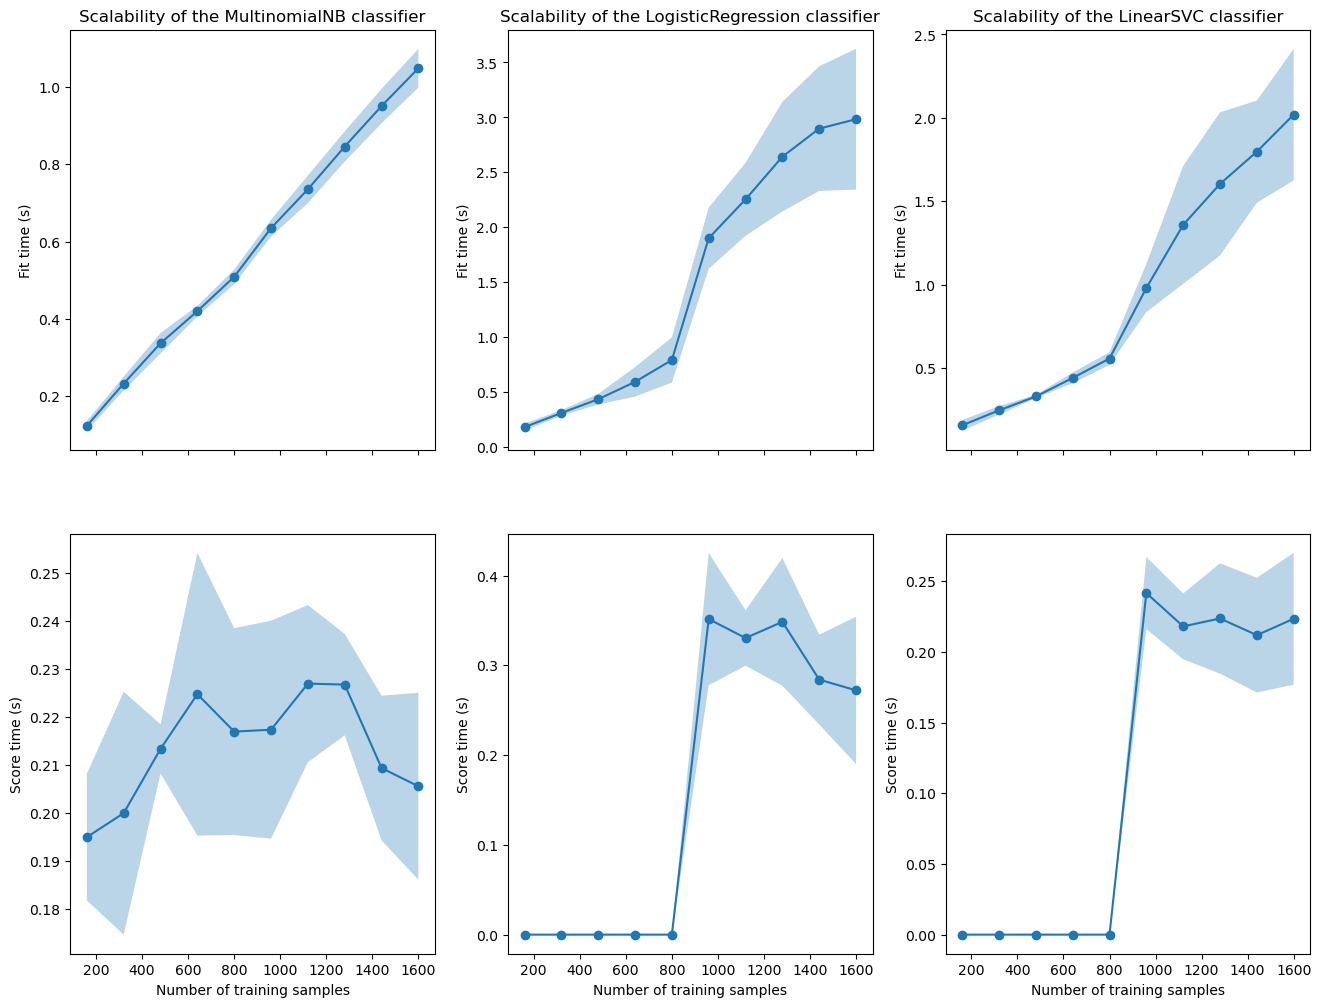
\includegraphics[width=\textwidth]{./src/movies/complexity_analysis_nsamples.png} 
    \caption{Evolutivité des classifieurs en fonction de la taille des données d'entrainement}
    \label{complexity_analysis_nsamples_movies}
\end{figure}

Nous constatons que l'évolutivité de nos 3 classificateurs est similaire à précédemment. Cependant, il est important de noter qu'il est impossible d'évaluer notre modèle avec peu de données d'entrainement, une fois de plus.

\begin{figure}[H]
    \centering
    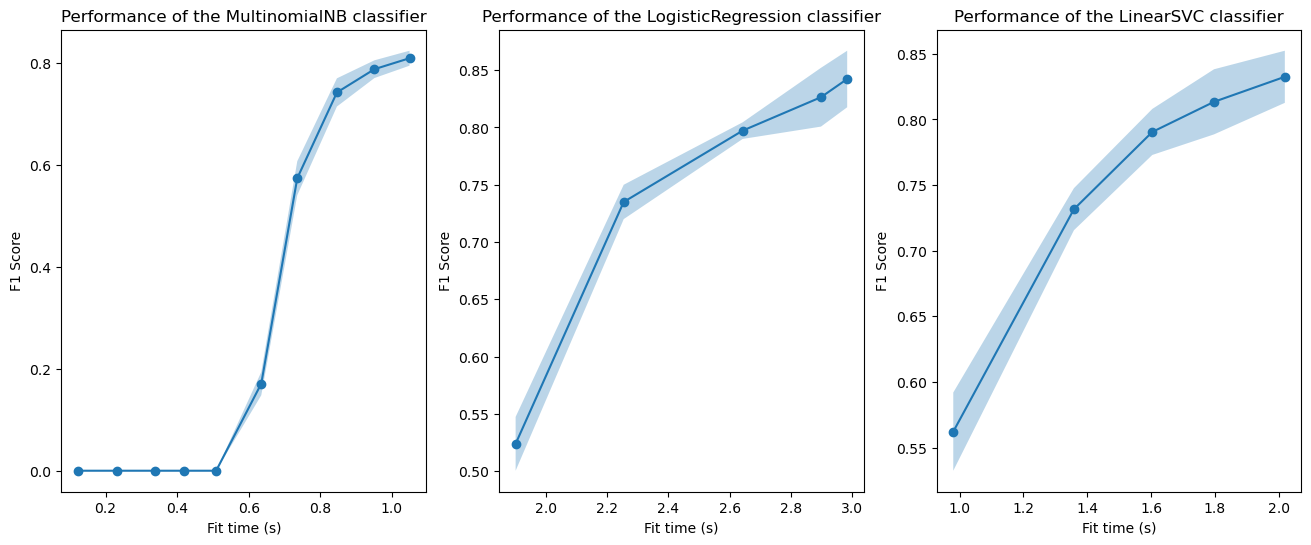
\includegraphics[width=\textwidth]{./src/movies/complexity_analysis_accuracy.png} 
    \caption{Performance des classifieurs}
    \label{complexity_analysis_accuracy_movies}
\end{figure}

Et enfin, on compare le temps d'apprentissage par rapport à la taille du vocabulaire utilisé. La taille du vocabulaire n'a de nouveau aucune influence sur la complexité du classifieur Bayésien naïf. Enfin, le SVM linéaire et la régression logistique ont des complexités similaires.

\begin{figure}[H]
    \centering
    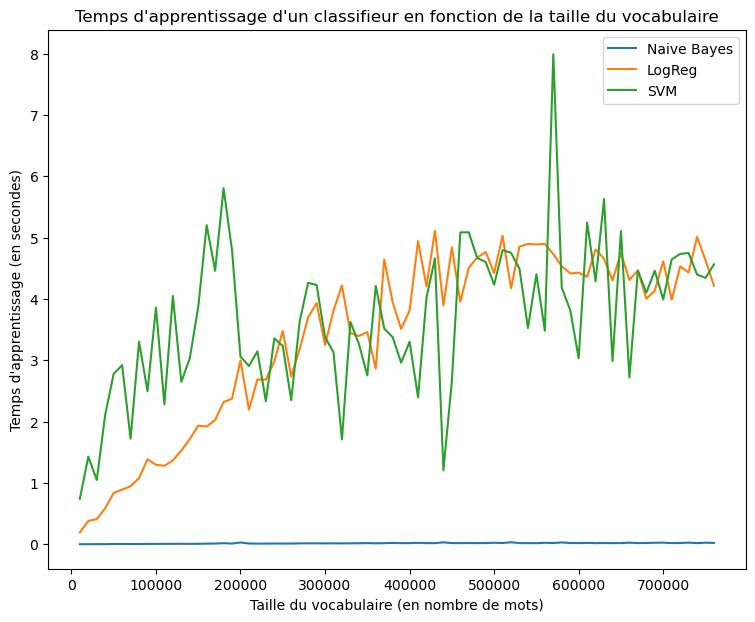
\includegraphics[width=0.6\textwidth]{./src/movies/complexity_analysis_vocabulary.png} 
    \caption{Evolutivité des classifieurs en fonction de la taille du vocabulaire}
    \label{complexity_analysis_vocabulary_movies}
\end{figure}

\subsubsection{Validation croisée}
Ici, nous utiliserons 8-fold en validation croisée pour évaluer nos modèles, le gain est léger mais plus stable par rapport à un 5-fold, tout en ayant un temps d'apprentissage similaire. Pour les mêmes raisons qu'évoquées que précédemment, le leave-one-out est trop coûteux.

\begin{figure}[H]
    \centering
    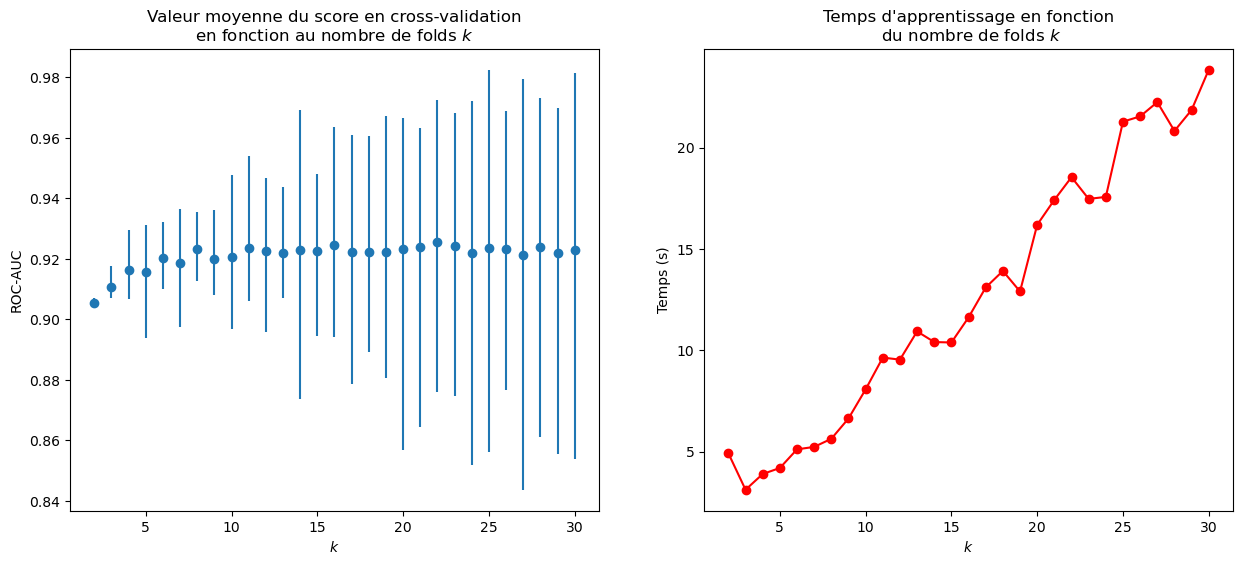
\includegraphics[width=\textwidth]{./src/movies/crossval_analysis.png} 
    \caption{Optimisation du nombre de folds}
    \label{crossval_analysis_movies}
\end{figure}

\paragraph{À quelles performances s'attendre ?} Sur une simple représentation par sac de mots, les performances sont plus que correctes ($> 90$), sans avoir paramétré notre modèle. La difficulté sera d'avoir un modèle qui généralise bien malgré un petit nombre de données d'entrainement.

\begin{figure}[H]
    \centering
    \includegraphics[width=\textwidth]{./src/movies/roc_curve.png} 
    \caption{Courbes ROC et Précision-Rappel en baseline}
    \label{roc_curve_movies}
\end{figure}

\subsection{Résultats et discussions}

Pour ce modèle nous avions envisagé plusieurs scénarios : en plus des $n$-grammes, nous nous sommes dit que regarder les caractères au lieu des mots pouvait être pertinente (\texttt{char\_wb}), du fait qu'on trouve souvent des mots similaires dans les classes. Néanmoins, le meilleur modèle est obtenu grâce à une représentation sac de mots binaires et des représentations (uni-gramme, bi-gramme) (en limitant le vocabulaire à 100~000), où les fréquences sont pondérées et le classifieur est un SVM linéaire où la fonction de coût est une hinge loss (avec un paramètre de régularisation très élevé). 

\begin{table}[H]
    \centering
    \begin{tabular}{ll}
        Paramètres & Valeurs \\ \hline
        CountVectorizer & binary=True, lowercase=False, max\_df=0.75, \\
        ~ & max\_features=100000, ngram\_range=(1, 2), strip\_accents='unicode' \\ 
        TfidfTransformer &  \\ 
        LinearSVC & C=448772.9166040199, loss='hinge' \\ 
    \end{tabular}
    \caption{Paramètre de la pipeline pour le SVM linéaire}
    \label{table:svmparams}
\end{table}

Après optimisation, on gagne quelques points en score. Pour un score de 0.90 en train, on obtient 0.85 en validation sur le serveur d'évaluation. Ci-après, les scores obtenus en tests sur la table \ref{table:logregmovies} et les courbes de score sur la figure \ref{roc_curve_opti}.

\begin{table}[H]
    \centering
    \begin{tabular}{lllll}
        precision & recall & f1-score & support & ~ \\ \hline
        0 & 0.91 & 0.88 & 0.90 & 189 \\ 
        1 & 0.90 & 0.92 & 0.91 & 211 \\ 
        accuracy & 0.90 & 400 & ~ & ~ \\ 
        macro avg & 0.90 & 0.90 & 0.90 & 400 \\ 
        weighted avg & 0.90 & 0.90 & 0.90 & 400 \\ 
    \end{tabular}
    \caption{Résultat détaillé pour le SVM linéaire}
    \label{table:logregmovies}
\end{table}

\begin{figure}[H]
    \centering
    \includegraphics[width=\textwidth]{./src/movies/roc_curve_opti.png} 
    \caption{Courbes ROC et Précision-Rappel, modèle optimisé}
    \label{roc_curve_opti}
\end{figure}

Et les features les plus importantes de notre modèle, qui ne sont que des bi-grammes :

\begin{figure}[H]
    \centering
    \includegraphics[width=\textwidth]{./src/movies/param_analysis_SVC.png}
    \caption{Top features, SVM linéaire}
    \label{features_svm_movies}
\end{figure}

\section{Ouverture}

Nous avons envisagé d'améliorer les performances des modèles de reconnaissance des locuteurs en utilisant des techniques d'embedding vectoriel, qui permettent de représenter chaque mot sous forme d'un vecteur de nombres réels.

Cependant, lors de nos expérimentations, nous avons constaté que l'utilisation d'un modèle d'embedding vectoriel n'a pas amélioré les performances de notre modèle Bag of Words, et même parfois les a détériorées. Nous pensons que cela est du notamment un choix inapproprié d'algorithme d'embedding ou peut être à une taille de corpus insuffisante pour entraîner le modèle d'embedding sur la classe minoritaire, ou encore une distribution de vocabulaire mal adaptée.

En fin de compte, nous avons décidé de ne pas creuser davantage cette solution et de poursuivre notre projet avec la technique de Bag of Words seule, qui a donné des performances satisfaisantes. Nous concluons que dans certains cas, l'utilisation d'un modèle d'embedding vectoriel n'est pas toujours la meilleure option pour améliorer les performances d'un modèle de NLP basé sur les Bag of Words, et qu'il est important de considérer chaque cas individuellement pour déterminer la meilleure approche à utiliser.

Nous avons également pensé à utiliser une mesure de confiance de la prédiction afin de pouvoir détecter les bordures de blocs et le bruit. A vu d'oeil, la confiance semblait assez peu consistante avec le bruit ou les débuts/fins des discours, ce qu'il fait que nous n'avons pas plus développer ce point.

Une autre piste était d'effectuer une réduction de dimension sur la matrice BoW comme en TME et de voir l'impact sur les performances des modèles.

\section{TME}

Au cours des quatre séances de TME de TAL, nous avons abordé plusieurs techniques importantes. 
Tout d'abord, nous avons appris comment pré-traiter les textes pour les rendre utilisables dans des modèles de traitement du langage naturel, en utilisant des techniques telles que la séparation en mots, la suppression de la ponctuation et des mots vides, et la création de matrices creuses pour représenter les données. 

Ensuite, nous avons étudié les modèles de Markov et les champs aléatoires conditionnels pour la modélisation de séquences, ainsi que les algorithmes de clustering tels que K-Means, LSA, pLSA et LDA pour regrouper des données similaires. 

Nous avons également exploré la classification de sentiments en utilisant Word2Vec et les modèles d'embedding de mots pour le traitement de séquences et l'étiquetage de parties du discours, en utilisant des modèles d'embedding de mots avec CRF. 

Enfin, nous avons abordé des sujets plus avancés tels que les réseaux de neurones récurrents (RNN) et les transformateurs pour le traitement de texte.

Toutes les idées de ce projet sont nées grâce aux enseignements dispensés lors des TMEs, tels que l'idée d'utiliser des modèles de Markov pour identifier des blocs de discours, la réduction de dimension, ou encore l'utilisation de techniques de Word Embedding. 

Ce fut un projet passionnant où, une fois immergés, de nombreuses possibilités se présentaient à nous, mais le temps imparti s'imposait également.

\end{document}
